% This is LLNCS.DEM the demonstration file of
% the LaTeX macro package from Springer-Verlag
% for Lecture Notes in Computer Science,
% version 2.4 for LaTeX2e as of 16. April 2010
%
\documentclass{llncs}
%
\usepackage{makeidx}  % allows for indexgeneration
%
\usepackage{times}
\usepackage{helvet}
\usepackage{courier}
\usepackage{tikz}
\usepackage{amssymb}
\usepackage{xspace}
\usepackage{amsmath}
\usepackage{algorithm}
\usepackage{algpseudocode}
%\usepackage{hyperref} % massively buggy on Tias' pc % Well, Tias' PC is a pile of crap
%\frenchspacing
\setlength{\pdfpagewidth}{8.5in}
\setlength{\pdfpageheight}{11in}
% \pdfinfo{
% /Title Sequence Mining with Constraint Based Solver. 
% /Subject (AAAI Publications)
% /Author (AAAI Press)}
%\setcounter{secnumdepth}{0} % Tias: why would we not have numbered sections?

\usepackage{adjustbox}

\newcommand{\Zinc}{\mbox{Zinc}\xspace}
\newcommand{\MiniZinc}{\mbox{MiniZinc}\xspace}
\newcommand{\MiningZinc}{\mbox{MiningZinc}\xspace}
\newcommand{\FlatZinc}{\mbox{FlatZinc}\xspace}
\usepackage{listings}

\newcommand{\todo}[1]{\framebox{{\large\bf TODO:~}{#1}}}
\newcommand{\D}{\ensuremath{D}}
\newcommand{\V}{\ensuremath{\mathcal V}}
\newcommand{\bigO}{\ensuremath{\mathcal O}}
\newcommand{\matchreg}{\ensuremath{match\mbox -regular}\xspace}
\newcommand{\maxcost}{\ensuremath{max\mbox -cost}\xspace}
\newcommand{\minweight}{\ensuremath{min\mbox -weight}\xspace}
\newcommand{\minsize}{\ensuremath{min\mbox -size}\xspace}
\newcommand{\maxgap}{\ensuremath{max\mbox -gap}\xspace}
\newcommand{\maxspan}{\ensuremath{max\mbox -span}\xspace}
\newcommand{\Maxgap}{\ensuremath{Max\mbox -gap}\xspace}
\newcommand{\Maxspan}{\ensuremath{Max\mbox -span}\xspace}
\newcommand{\discriminant}{\ensuremath{discriminant}\xspace}
\newcommand{\posmatch}{\ensuremath{position\mbox -match}\xspace}
\newcommand{\Posmatch}{\ensuremath{Position\mbox -match}\xspace}
\newcommand{\isemb}{\ensuremath{is\mbox -embedding}\xspace}
\newcommand{\Isemb}{\ensuremath{Is\mbox -embedding}\xspace}

\newcommand{\optional}[1]{} % to hide optional text to fit the page limit
\newcommand{\subsubspace}{\vspace*{-0.8em}} % for subsubsections (need to do manually)
\newcommand{\parspace}{\vspace*{-0.4em}} % for paragraphs (need to do manually)

\newcommand{\var}{\bf}
\newcommand{\surl}[1]{{\footnotesize\url{#1}}}
\newcommand{\seq}[1]{{\ensuremath{\mathrm {\langle \lit{#1} \rangle}}}\xspace} % A sequence 
\newcommand{\lit}[1]{{\ensuremath{\mathrm {\lowercase{#1}}}}\xspace}
\renewcommand{\equiv}{\Longleftrightarrow}
% \lstset{basicstyle=\ttfamily,columns=fixed}
\lstset{basicstyle=\small\sffamily,columns=fixed}

\lstdefinelanguage{zinc} 
  {morekeywords={declarative programming, sequence mining, sequence mining, episode mining, serial episode mining, pattern mining, constraint programming, constrained pattern mining}
  ,classoffset=1
  ,sensitive=false
  ,comment=[l]{\%}
  ,morecomment=[l]{//}
  ,morecomment=[s]{/*}{*/}
  ,morestring=[b]"
  ,literate=
  }


\begin{document}
\title{Constraint-based sequence mining\\using constraint programming\protect\footnote{This paper is published at CPAIOR 2015, this arxiv version additionally has an appendix.}}


\author{Benjamin Negrevergne \and Tias Guns}
\authorrunning{B. Negrevergne and T. Guns} % abbreviated author list (for running head)
\institute{DTAI Research group,\\ KU Leuven\\
  \email{\{firstname\}.\{lastname\}@cs.kuleuven.be}
  % \and
  % LIRMM, University Montpellier~2,\\
  % Montpellier, France\\
  % \email{coletta@lirmm.fr}
}


\maketitle
\begin{abstract}
% Developing generic pattern mining methods that support a wide range of user-supplied constraints is a major challenge. In this paper, we build on recent successes in the use of constraint programming for pattern mining, and investigate the class of sequence mining problems (also known as a serial episode mining). 

The goal of constraint-based sequence mining is to find sequences of symbols that are included in % (i.e. that are subsequences of)
a large number of input sequences and that satisfy some constraints specified by the user. Many constraints have been proposed in the literature, but a general framework is still missing. We investigate the use of constraint programming as general framework for this task.

We first identify four categories of constraints that are applicable to sequence mining. We then propose two constraint programming formulations.  The first formulation introduces a new global constraint called {\em exists-embedding}. This formulation is the most efficient but does not support one type of constraint. To support such constraints, we develop a second formulation that is more general but incurs more overhead. Both formulations can use the projected database technique used in specialised algorithms.% , and can use \textit{projected frequency} to speed up the search.

%Computationally, we show how our formulation relates to the concept of projected databases in specialised algorithms, and that we can use the related concept of local frequency to speed up the search in both formulations. Experiments demonstrate the runtime behaviour 

%We study the computational properties of the proposed formalisations and observe that the use of global constraints and specialised search strategies is essential to  make more constrained settings practical in a generic CP system.
Experiments demonstrate the flexibility towards constraint-based settings and compare the approach to existing methods.
% Finally, we discuss  the benefits and limitations of a CP-based approach for sequence mining.

  \keywords{sequential pattern mining, sequence mining, episode mining, constrained pattern mining, constraint programming, declarative programming}
\end{abstract}

%{\bf limit for long papers is 15 LNCS pages *plus references*.}


\section{Introduction} \label{sec:intro}
In AI in general and in data mining in particular, there is an increasing interest in developing general methods for data analysis. In order to be useful, such methods should be easy to extend with domain-specific knowledge. %These methods can then be used directly by the domain experts to update and refine their knowledge about the problem.

In pattern mining, the frequent sequence mining problem has already been studied in depth, but usually with a focus on efficiency and less on generality and extensibility. An important step in the development of more general approaches was the cSpade algorithm~\cite{zaki2000sequence} which supports a variety constraints.
% Tias: If this is general motivation, put it before discussion one concrete paper
% Tias: If it is to motivate this particular paper: that looks weird
%Such constraints can be used to extend the basic sequence mining task into more complex and interesting mining tasks.
It supports many constraints such as constraints on the length of the pattern, on the maximum gap in embeddings or on the discriminative power of the patterns between datasets.
% Tias: 'since then', zaki was not the first, tricky and should not become related work section here?
%Since then, several other algorithms have been extended to support constraints (E.g. \cite{OhtaniKUA09}).
Many other constraints have been integrated into specific mining algorithms (e.g. \cite{han2001prefixspan,yan2003clospan,wang2004bide,OhtaniKUA09}).
However, none of these are truly generic in that adding extra constraints usually amounts to changing the data-structures used in the core of the algorithm. %(implementation).


% One major development has been the concept of projected databases for patterns that share a prefix~\cite{han2001prefixspan} (or suffix~\cite{zaki2000sequence}). These can be used to compute the \textit{local frequency} of individual symbols and avoid extending the prefix into an infrequent pattern.
% These algorithms have also been extended to support specific constraints such as regular expressions~\cite{DBLP:conf/vldb/GarofalakisRS99} or only mining closed patterns~\cite{yan2003clospan,wang2004bide}. 



%Building on the work by \cite{DeReadt08} several publications have addressed the problem of mining patterns in sequences with generic solvers. These  publications improve the state of the art by proposing a problem formulation in a given framework such as CP, SAT or Answer Set Programming as well as the formulation of a variety of constraints that can be added to the base problem formulation. The gain in generality usually comes at the expense of a lower efficiency.

For \textit{itemset} mining, the simplest form of pattern mining, it has been shown that constraint programming (CP) can be used as a generic framework for constraint-based mining~\cite{cp4im_aij} and beyond~\cite{DBLP:conf/cpaior/RojasBLCL14,dominance_dp}. %Other works have built on this work and extended the range of constraints that can be handled to pattern sets~\cite{cp4im_pakdd11,nary_cp}, sky-patterns~\cite{DBLP:conf/cpaior/RojasBLCL14} and general pairwise constraints over patterns~\cite{dominance_dp}.
%
Recent works have also investigated the usage of CP-based approaches for mining sequences with explicit wildcards~\cite{coquery2012sat,JSS-13-3,kemmarictai}. A wildcard represents the presence of exactly one arbitrary symbol in that position in the sequence. 

The main difference between mining itemsets, sequences with wildcards and standard sequences lies in the complexity of testing whether a pattern is included in another itemset/sequence, e.g. from the database. For itemsets, this is simply testing the subset inclusion relation which is easy to encode in CP. For sequences with wildcards and general sequences, one has to check whether an \textit{embedding} exists (matching of the individual symbols). But in case only few embeddings are possible, as in sequences with explicit wildcards, this can be done with a disjunctive constraint over all possible embeddings \cite{kemmarictai}. In general sequence (the setting we address in this paper), a pattern of size $m$ can be embedded into a sequence of size $n$ in $O(n^m)$ different ways, hence prohibiting a direct encoding or enumeration. 

%Metivier et al.~\cite{metivierconstraint} have studied this problem in a constraint programming setting before. They used an automaton to encode all possible embeddings, and use the \textit{regular} global constraint to check whether an embedding exists. Other constraints such as item, size, gap and closedness constraints can be combined with this setting. In this work, we do not use automata but investigate a specialised global constraint as well as a decomposition that exposes variables corresponding to an embedding.

The contributions of this paper are as follows: 
\begin{itemize} %\addtolength{\itemsep}{-0.6\baselineskip}
\item %\vspace{-0.4em}
      We present four categories of user-constraints, this categorization will be useful to compare the generality of the two proposed models. 
\item We introduce an {\em exists-embedding} global constraint for sequences, and show the relation to projected databases and \textit{projected frequency} used in the sequence mining literature to speedup the mining process \cite{han2001prefixspan,zaki2001spade}. 
\item We propose a more general formulation using a decomposition of the {\em exists-embedding} constraint. Searching whether an embedding exists for each transaction is not easily expressed in CP and requires a modified search procedure. %While supporting more constraints, specialised search over the embedding variables has to be used to be correct under arbitrary constraints.
\item We investigating the effect of adding constraints, and compare our method with state-of-the-art sequence mining algorithms.
\end{itemize}
%\vspace{-0.4em}

%The main insight in this paper is a trade-off between the extensible of a model and the complexity of the solving strategy.  We believe that the limits identified in this paper and the proposed workarounds can be used as insights to devise a more principled CP-based approach for mining sequences.

\noindent The rest of the paper is organized as follows: Section~\ref{sec:preliminaries} formally introduces the sequence mining problem and the constraint categories. Section~\ref{sec:seq_cp} explains the basics of encoding sequence mining in CP. Section~\ref{sec:first-model} and \ref{sec:second-model} present the model with the global constraint and the decomposition respectively. Section~\ref{sec:experiments} presents the experiments. After an overview of related work (Section~\ref{sec:related}), we discuss the proposed approach and results in Section~\ref{sec:conclusions}.


\section{Sequence mining}
\label{sec:preliminaries}


Sequence mining~\cite{agrawal1995mining} can be seen as a variation of the well-known itemset mining problem proposed in \cite{agrawal1994fast}. In itemset mining, one is given a set of \textit{transactions}, where each transaction is a set of items, and  the goal is to find  patterns (i.e. sets of items) that are included in a large number of transactions.  In sequence mining, the problem is similar except that both transactions and patterns are ordered, (i.e. they are sequences instead of sets) and symbols can be repeated. 
% In sequence mining each transaction is assumed to be ordered; it is a sequence of symbols from a given alphabet, where symbols can be repeated. The goal is to find a sequence, a sequence of symbols, which is a subsequence of a sufficient amount of transactions.
%
For example, $\seq{b,a,c,b}$ and $\seq{a,c,c,b,b}$ are two sequences, and the sequence $\seq{a,b}$ is one possible pattern included in both.

%Fig. \ref{fig:embedding} shows two transactions $T_1$ and $T_2$ and a a simple sequence mining example in which the pattern $S = \seq{AB}$ is included in two  transactions $T_1$ and $T_2$.
This problem is known in the literature under multiple names, such as {\em embedded subsequence mining}, {\em sequential pattern mining}, {\em flexible motif mining}, or {\em serial episode mining} depending on the application.


\subsection{Frequent sequence mining: problem statement}
\label{sec:freq-sequ-mining}
%\vspace{-0.2em}
A key concept of any pattern mining setting is the pattern inclusion relation. % is when a pattern is considered to be included in a transaction, also called the inclusion relation.
In sequence mining, a pattern is included in a transaction if there exists an embedding of that sequence in the transaction; where an embedding is a mapping of every symbol in the pattern to the same symbol in the transaction such that the order is respected. %list of increasing positions that for every symbol in the pattern indicates where it can be matched in the transaction.

\begin{definition}[Embedding in a sequence]
  \label{def:seq-embedding}
  Let $S = \langle s_1,\ldots, s_m \rangle$ and $S' = \langle s'_1, \ldots, s'_n\rangle$ be two sequences of size $m$ and $n$ respectively with $m\leq n$. The tuple of integers $e = (e_1, \ldots, e_m)$ is an \textbf{embedding} of $S$ in $S'$  (denoted $S \sqsubseteq_e S'$) if and only if:
  %\vspace{-0.5em}
  \begin{align}
    S \sqsubseteq_e S' \leftrightarrow e_1 < \ldots < e_m ~\mbox{and}~ \forall i \in 1,\ldots,m: s_i = s'_{e_i}
  \end{align}
  %\begin{itemize}
  %\item $\forall i \in 1,\ldots, n,\hspace{1em} e_1 < \ldots < e_n$; and
  %\item $\forall i \in 1,\ldots,n,\hspace{1em} s_i = s'_{e_i}$
  %\end{itemize}
\end{definition}
For example, let $S=\seq{a,b}$ be a pattern, then $(2,4)$ is an embedding of $S$ in $\seq{b,a,c,b}$ and $(1,4),(1,5)$ are both embeddings of $S$ in $\seq{a,c,c,b,b}$. An alternative %sequence mining 
setting considers sequences of \textit{itemsets} instead of sequences of individual symbols. In this case, the definition is $S \sqsubseteq_e S' \leftrightarrow e_1 < \ldots < e_n ~\mbox{and}~ \forall i \in 1,\ldots,n: s_i \subseteq s'_{e_i}$. We do not consider this setting further in this paper, though it is an obvious extension.

We can now define the sequence inclusion relation as follows:
\begin{definition}[Inclusion relation for sequences]
  \label{def:seq-incl-rel}
  Given two sequences $S$ and $S'$, $S$ \textbf{is included in} $S'$ (denoted $S \sqsubseteq S'$) if there exists an embedding $e$ of $S$ in $S'$:
  %\vspace{-0.5em}
  \begin{align} \label{eq:sec-incl-rel}
    S \sqsubseteq S' \leftrightarrow \exists e ~\mbox{s.t.}~ S \sqsubseteq_e S'.
  \end{align}
   %there exist at least one embedding $e$ such that $$.
\end{definition}
To continue on the example above, $S=\seq{a,b}$ is included in both $\seq{b,a,c,b}$ and $\seq{a,c,c,b,b}$ but not in $\seq{c,b,a,a}$.
 
%\begin{figure}
%  \centering
%  \begin{large}
%      \begin{tikzpicture}[scale=0.7, transform shape]
%        \tikzstyle{seq_item}=[draw, fill=blue!20, shape=rectangle, minimum size=1cm];
%        \tikzstyle{seq_item_static}=[draw, fill=white, shape=rectangle, minimum size=1cm];
%        \tikzstyle{match}=[out=90, in =270, thick, -latex, color=red!80!black];
%            \newcounter{x}
%
%        \node at (0, -3.5) {$S$}; 
%        \setcounter{x}{1}
%        \foreach \i in {\lit A, \lit B}{
%          \node[seq_item] at (\arabic{x}, -3.5) (p\arabic{x}) {\textbf{\i}};
%          \stepcounter{x}
%        }
%
%
%        \node at (0, 0) {$T_1$}; 
%        \setcounter{x}{1}
%        \foreach \i in {\lit B, \lit A, \lit C, \lit B}{
%          \node[seq_item_static] at (\arabic{x}, 0) (t1\arabic{x}) {\textbf{\i}};
%          \stepcounter{x}
%        }
%
%        \node at (0, -1.1) {$T_2$}; 
%        \setcounter{x}{1}
%        \foreach \i in {\lit A, \lit C, \lit C, \lit B}{
%          \node[seq_item_static] at (\arabic{x}, -1.2) (t2\arabic{x}) {\textbf{\i}};
%          \stepcounter{x}
%        }
%
%
%          % \draw (p1.265) edge[thick,-latex, color=blue!80!black] (t11.95);
%          % \draw (p2) edge[thick,-latex, color=blue!80!black] (t12);
%
%        \draw (p1) edge[match] (t12);
%        \draw (p2) edge[match] (t14);
%
%        \draw (p1) edge[match, dashed] (t21);
%        \draw (p2) edge[match, dashed] (t24);
%
%        % \node[seq_item] (a) {A} ;space
%        \end{tikzpicture}
%        \end{large}
%\caption{Sequence $S = \seq{AB}$ is included in transaction $T_1$ (solid arrows) and transaction $T_2$ (dashed arrows).}
%\label{fig:embedding}
%\end{figure}


\begin{definition}[Sequential dataset]
  Given an alphabet of symbols $\Sigma$, a {\em sequential dataset} $D$ is a multiset of sequences defined over symbols in $\Sigma$. 
\end{definition}
Each sequence in $D$ is called a {\em transaction} using the terminology from itemset mining. The number of transactions in $D$ is denoted $|D|$ and the sum of the lengths of every transaction in $D$ is denoted $||D||$ ($||D|| = \sum_{i = 1}^{|D|}|T_i|$).
Furthermore, we use {\em dataset} as a shorthand for {\em sequential dataset} when it is clear from context. 


Given a dataset $D = \{T_i, \ldots, T_n\}$, one can compute the {\bf cover} of a sequence $S$ as the set of all transactions $T_i$ that contain $S$:
%\vspace{-0.5em}
\begin{equation}
  \label{eq:cover}
cover(S, \D) = \{T_i \in \D : S \sqsubseteq T_i\}
\end{equation}


We can now define frequent sequence mining, where the goal is to find all patterns that are frequent in the database; namely, the size of their cover is sufficiently large.

\begin{definition}[Frequent sequence mining]
\label{def:spm}
Given:
\begin{enumerate}
%\vspace{-0.4em}
\item an alphabet $\Sigma$ 
\item a sequential dataset $\D = \{T_1, \ldots, T_{n}\}$ defined over $\Sigma$ % an alphabet $\Sigma$: $X_i = \langle s_1,{\ldots},s_{|X_i|}\rangle$ with $\forall s_j: s_j \in \Sigma$. 
\item a minimum frequency threshold $\theta$,
\end{enumerate}
%\vspace{-0.5em}
\noindent enumerate all sequences $S$ %of symbols in $\Sigma$
such that
%\begin{align}
%\label{eq:cminfreq}
$
  |cover(S, \D)| \ge \theta  
$.
%\end{align}
\end{definition}%

% We now give an overview of constraints that can be added to the frequent sequence mining problem.
In large datasets, the number of frequent sequences is often too large to be analyzed by a human. Extra constraints can be added to extract fewer, but more relevant or interesting patterns. Many such constraints have been studied in the past.

%\vspace{-0.5em}
\subsection{Constraints}
\label{sec:constraints-max-1}
%\vspace{-0.2em}

Constraints typically capture background knowledge and are provided by the user. We identify four categories of constraints for sequence mining: 1) constraints over the pattern, 2) constraints over the cover set, 3) constraints over the inclusion relation and 4) preferences over the solution set. %We detail these categories and give example in the following sections. 


\subsubspace
\subsubsection{Constraints on the pattern}
%This type of constraint 
These put restrictions on the structure of the pattern. Typical examples include size constraints %, weight constraints 
or regular expression constraints.\\
{\em Size constraints:}
A size constraint is simply $|S| \gtrless \alpha$ where $\gtrless \in \{=,\neq,>,\geq,<,\leq\}$ and $\alpha$ is a user-supplied threshold. It is used to discard  small patterns.\\
%
% {\em Weight constraints.} 
% Given a cost function $w: \Sigma \rightarrow \mathbb R$, that maps every symbol in $\Sigma$ to a real-valued weight. Weight constraints are of the form $\sum_{s \in S} w(s) \gtrless \alpha$.
% %Weight constraints are useful in many application. For example in natural language processing, words can be weighted with idf values ({\em inverse document frequency}) which indicate the relevance of each word in a collection of document. The $\minweight$ constraint can then be used to extract the sentences made of  the most relevant words. 
% %
{\em Item constraints:} One can constrain a symbol $t$ to surely be in the pattern: $\exists s \in S: s = t$; or that it can not appear in the pattern: $\forall s \in S: s \neq t$, or more complex logical expressions over the symbols in the pattern.\\
{\em Regular expression constraints:}
Let $R$ be a regular expression over the vocabulary $V$ and $L_R$ be the language of sequences recognised by $R$, then for any sequence pattern $S$ over $V$, the {\em \matchreg} constraint requires that $S \in L_R$~\cite{han2001prefixspan}.

\subsubspace
\subsubsection{Constraints on the cover set.}
The {\em minimum frequency} constraint $|cover(S,D)| \geq \theta$ is the most common example of a constraint over the cover set. Alternatively, one can impose the {\em maximum frequency} constraint: $|cover(S,D)| \leq \beta$\\ % , or different frequency constraints on different datasets for the same pattern.
%
{\em Discriminating constraints:} In case of multiple datasets, discriminating constraints require that patterns effectively distinguish the datasets from each other. 
Given two datasets $D_1$ and $D_2$, one can require that the ratio between the size of the cover of both is above a threshold: $\frac{|cover(S,D_1)|}{|cover(S,D_2)|} \geq \alpha$. Other examples include more statistical measures such as information gain and entropy~\cite{correlated_cp}.

%\paragraph{Discriminating constraint:}
%Given a labeling function $l: T \rightarrow \{0, 1\}$ that maps each transaction to a label $0$ or $1$, we can define the {\em discriminating} as a constraint over a cover set $C$ as follows. 
%\begin{equation}
%  \label{eq:cdiscriminating}
%  discriminating_{l}(C) \equiv \left\{ \frac{ |\{ T \in C \mid l(T) = 1 \}|}{|\{ T \in C \mid l(T) = 0 \}|} \right\} \ge \rho
%\end{equation}

\subsubspace
\subsubsection{Constraints over the inclusion relation.}
The inclusion relation in definition~\ref{def:seq-incl-rel} states that $S \sqsubseteq S' \leftrightarrow \exists e ~\mbox{s.t.}~ S \sqsubseteq_e S'$. Hence, an embedding of a pattern can match symbols that are far apart in the transaction. For example, the sequence $\seq{a,c}$ is embedded in the transaction $\seq{a,b,b,b,\ldots,b,c}$ independently of the distance between $\lit a$ and $\lit c$ in the transaction. This is undesirable when mining datasets with long transactions. The \maxgap and \maxspan constraints  \cite{zaki2000sequence}  impose a restriction on the embedding, and hence on the inclusion relation. %{\em $Max\mbox -gap$ constraint:}
\label{sec:maxgap-constraint}
The {\em \maxgap constraint} is satisfied on a transaction $T_i$ if an embedding $e$ maps every two consecutive symbols in $S$ to symbols in $T_i$ that are close to each-other: $\maxgap_i(e) \Leftrightarrow \forall{j \in 2..|T_i|}, (e_{j} - e_{j-1} - 1) \le \gamma$.
For example,  the sequence $\seq{abc}$ is embedded in the transaction \seq{adddbc} with a maximum gap of 3 whereas \seq{ac} is not.
%
%{\em $Max\mbox -span$ constraint:}
\label{sec:maxspan-constraint}
The {\em \maxspan constraint} requires that the distance between the first and last position of the embedding of all transactions $T_i$ is below a %user defined
threshold~$\gamma$: 
%\begin{equation}
%  \label{eq:cmaxspan}
$
  \maxspan_i(e) \Leftrightarrow e_{|T_i|} - e_1 + 1 \le \gamma
$.
%\end{equation}

\subsubspace
\subsubsection{Preferences over the solution set.}
A pairwise preference over the solution set expresses that a pattern $A$ is preferred over a pattern $B$. In~\cite{dominance_dp} it was shown that condensed representations like closed, maximal and free patterns can be expressed as pairwise preference relations. Skypatterns~\cite{DBLP:conf/cpaior/RojasBLCL14} and multi-objective optimisation can also be seen as preference over patterns. As an example, let $\Delta$ be the set of all patterns; then, the set of all closed patterns is $\{S \in \Delta | \nexists S' \mbox{ s.t. } S \sqsubset S' \mbox{ and } cover(S,\D) = cover(S',\D)\}$.

%The closed constraint can be defined as follows. 
%\begin{equation}
%  \label{eq:closed}
%    closed(S) \equiv \nexists S' \mid S \sqsubset S' \mbox{ and } cover(S,\D) = cover(S',\D)
%\end{equation}
%\todo{I don't know how to write this as a constraint}

%The maximal constraint can be defined as follows. 
%\begin{equation}
%  \label{eq:closed}
%  maximal(S) \equiv \nexists S' \mid S \sqsubset S'
%\end{equation}


% \subsection{A general constraint-based framework?}

% No framework exists that supports all of these constraints. For itemsets, constraint programming has proven to be a framework in which constraints of type 1, 2 and 4 (for itemsets specifically) can be expressed. Type 3 constraints are not relevant for itemsets as the cover relation is simply the subset relation, so there is no explicit notion of an \textit{embedding}.

% In this paper, we will investigate a constraint programming based framework that can support all of these constraints, and we will study the computational properties (and limitations) of this framework.

%\vspace{-0.2em}
\section{Sequence Mining in Constraint Programming}\label{sec:seq_cp}
%\vspace{-0.2em}
%Constraint Programming is a methodology for solving Constraint Satisfaction and Optimisation problems. Formally, a CSP is 
In constraint programming, problems are expressed as a constraint satisfaction problem (CSP), or a constraint optimisation problem (COP). A CSP $X=(V,D,C)$ consists of a set of variables $V$, a finite domain $D$ that defines for each variable $v \in V$ the possible values that it can take, and a set of constraints $C$ over the variables in $V$.  A solution to a CSP is an assignment of each variable to a value from its domain such that all constraints are satisfied. A COP additionally consists of an optimisation criterion $f(V)$ that expresses the quality of the solution. 

There is no restriction on what a constraint $C$ can represent.  Examples include logical constraints like ${\var X} \wedge {\var Y}$ or ${\var X} \rightarrow {\var Y}$ and mathematical constraints such as ${\var Z} = {\var X} + {\var Y}$ etc. Each constraint has a corresponding \textit{propagator} that ensures the constraint is satisfied during the search. Many \textit{global constraints} have been proposed, such as \textit{alldifferent}, which have a custom propagator that is often more efficient then if one would \textit{decompose} that constraint in terms of simple logical or mathematical constraints. A final important concept used in this paper is that of \textit{reified constraints}. A reified constraint is of the form ${\var B} \leftrightarrow C'$ where ${\var B}$ is a Boolean variable which will be assigned to the truth value of constraint $C'$. Reified constraints have their own propagator too.

\parspace
\paragraph{Variables and domains for modeling sequence mining.}
Modeling a problem as a CSP requires the definition of a set of variables with a finite domain, and a set of constraints. One solution to the CSP will correspond to one pattern, that is, one frequent sequence.

We model the problem using an array ${\var S}$ of integer variables representing the characters of the sequence and an array ${\var C}$ of Boolean variables representing which transactions include the pattern. This is illustrated in Fig. \ref{fig:principle1}:
%\vspace{-0.2em}
%
\begin{figure}[t]
  \centering
  \Large
      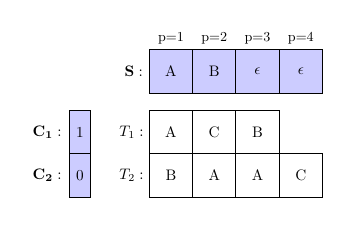
\begin{tikzpicture}[scale=0.55, transform shape]
        \tikzstyle{seq_item}=[draw, fill=blue!20, shape=rectangle, minimum size=1cm];
        \tikzstyle{seq_item_small}=[draw, fill=blue!20, shape=rectangle, minimum size=1cm, minimum width=0.5cm];
        \tikzstyle{seq_item_static}=[draw, fill=white, shape=rectangle, minimum size=1cm];
        \tikzstyle{myedge}=[thick, -latex, color=red!80!black];
        % \foreach \i/\x in {A/0, B/1, A/3 }{
        % \node[seq_item] at (\x, 0) (\i) {\i};
        % }
        \newcounter{y}

        % S var
        \node at (0.2, 0) {${\var S}:~$}; 
        \setcounter{y}{1}
        \foreach \i in {A, B, $\epsilon$, $\epsilon$}{
          \node[seq_item, label=above:{\small p=\arabic{y}}] at (\arabic{y}, 0) (j\arabic{y}) {\i};
          \stepcounter{y}
        }

        % T_1 var
        \node[seq_item_small] (t1) at (-1.1, -1.4) {$1$};
        \node at (-1.8, -1.4) {${\var C_1}:~$};
                
        % X_1 data
        \node at (0.15, -1.4) {$T_1:~$}; 
        \setcounter{y}{1}
        \foreach \i in {A, C, B}{
          \node[seq_item_static] at (0+\arabic{y}, -1.4) (x1\arabic{y}) {\i};
          %label=above:{\scriptsize x=\arabic{y}}
          \stepcounter{y}
        }
                
        % OH THE SHAMEFUL COPY/PASTE... (see me care)
        % T_2 var
        \node[seq_item_small] (t2) at (-1.1, -2.4) {$0$};
        \node at (-1.8, -2.4) {${\var C_2}:~$};
                
        % X_2 data
        \node at (0.15, -2.4) {$T_2:~$}; 
        \setcounter{y}{1}
        \foreach \i in {B, A, A, C}{
          \node[seq_item_static] at (0+\arabic{y}, -2.4) (x2\arabic{y}) {\i};
          \stepcounter{y}
        }
               
        %\node at (1, -3.4) {$\vdots$};        
        \end{tikzpicture}
\caption{Example assignment; blue boxes represent variables, white boxes represent data.}
\label{fig:principle1}  
%\vspace{-0.2em}
\end{figure}%
%
\begin{enumerate}
\item $T_1$ and $T_2$ represent two transactions given as input. We denote the number of transactions by $n$;
\item The array of variables ${\var S}$ represents the sequence pattern.
  Each variable ${\var S_j}$ represents the character in the $j$th position of the sequence.
  The size of ${\var S}$ is determined by the length of the longest transactions (in the example this is $4$).
  We want to allow patterns that have fewer than $max_i(|T_i)$ characters, hence we use $\epsilon$ to represent an unused position in ${\var S}$.
  The domain of each variable ${\var S_j}$ is thus $\Sigma \cup \{\epsilon\}$;
\item Boolean variables ${\var C_i}$ represent whether the pattern is included in transaction $T_i$, that is, whether ${\var S} \sqsubseteq T_i$. In the example, this is the case for $T_1$ but not for $T_2$.
\end{enumerate}

What remains to be defined is the constraints. The key part here is how to model the inclusion relation; that is, the constraint that verifies whether a pattern is included in the transaction. Conceptually, this is the following reified constraint: ${\var C_i} \leftrightarrow \exists e ~\mbox{s.t.}~ {\var S} \sqsubseteq_e T_i$.
%
As mentioned in the introduction, the number of possible embeddings is exponential in the size of the pattern. Hence, one can not model this as a disjunctive constraint over all possible embeddings (as is done for sequences with explicit wildcards~\cite{kemmarictai}).

% The solution proposed in~\cite{metivierconstraint} is to encode all possible embeddings of a transaction $T_i$ in a non-deterministic automaton with $|T_i|$ states (one for each position) and $|T_i|!$ transitions. The \textit{regular} global constraint is then used to check whether an embedding of the pattern exists. 
We propose two approaches to cope with this problem: one with a global constraint that verifies the inclusion relation directly on the data, % instead of building an automaton;
and one in which the inclusion relation is decomposed and the embedding is exposed through variables.

\section{Sequence mining with a global \textit{exists-embedding} constraint}
\label{sec:first-model}

The model consists of three parts: encoding of the pattern, of the minimum frequency constraint and finally of the inclusion relation using a global constraint.

\parspace
\paragraph{Variable-length\ pattern:} The array ${\var S}$ has length $k$; patterns with $l < k$ symbols are represented with $l$ symbols from $\Sigma$ and $(k - l)$ times an $\epsilon$ value. To avoid enumerating the same pattern with $\epsilon$ values in different positions, $\epsilon$ values can only appear at the end: %, that is they can not appear in between non-$\epsilon$ characters:
%\vspace{-0.2em}
  \begin{equation}
    \label{eq:well-formed}
    \begin{gathered}
          \forall j \in 1..(k-1): {\var S_{j}} = \epsilon \rightarrow {\var S_{j+1}} = \epsilon
    \end{gathered}
  \end{equation}
\optional{
This can be encoded with $k-1$ auxiliary variables and reified ${\var B} \leftrightarrow {\var S_j} = \epsilon$ constraints, and $1$ lexicographic 'less than or equal' constraint over the array of auxiliary variables (using the observation that ${\var B_1} \rightarrow {\var B_2} \equiv {\var B_1} \leq {\var B_2}$ for Boolean variables).
}

\parspace
\parspace
\paragraph{Minimum frequency:} At least $\theta$ transactions should include the pattern. This inclusion is indicated by the array of Boolean variables ${\var C}$:
%\vspace{-0.2em}
\parspace
  \begin{equation}
    \label{eq:minfreq}
    \begin{gathered}
        \sum_{i = 1}^n {\var C_i} \geq \theta
    \end{gathered}
  \end{equation}
\optional{
This can be encoded with $1$ linear inequality constraint over the ${\var C}$ variables.
}

\parspace
\parspace
\paragraph{Global exists-embedding constraint:}
The goal is to encode the relation:
$
{\var C_i} \leftrightarrow \exists e ~\mbox{s.t.}~ {\var S} \sqsubseteq_e T_i.
$
%
\begin{algorithm}[t]
\algtext*{EndIf}% Remove "end if" text
  \footnotesize %\scriptsize
\caption{Incremental propagator for ${\var C_i} \leftrightarrow \exists e ~\mbox{s.t.}~ {\var S} \sqsubseteq_e T_i$:\label{alg:global_emp}}
\textit{internal state, $pos_S$: current position in ${\var S}$ to check, initially 1}\\
\textit{internal state, $pos_e$: current position in $T_i$ to match to, initially 1}
\begin{algorithmic}[1]
\While{$pos_S \leq |T_i|$ and ${\var S}$[$pos_S$] is assigned\label{a1:while}} \Comment{note that $|T_i| \leq |{\var S}|$} % but symbols past $|X_i|$ must not be matched}
\If{${\var S}$[$pos_S$] $\neq \epsilon$}\label{a1:neq_eps}
\While{not ($T_i[pos_e] = {\var S}[pos_S])$ and $pos_e \leq |T_i|$\label{a1:while2}} \Comment find match
\State{$pos_e \gets pos_e + 1$}
\EndWhile
\If{$pos_e \leq |T_i|$} \Comment match found, on to next one
\State{$pos_S \gets pos_S + 1$; $pos_e \gets pos_e + 1$}
\Else
\State propagate ${\var C_i} = False$ and return
\EndIf
\Else \Comment previous ones matched and rest is $\epsilon$
\State propagate ${\var C_i} = True$ and return  \label{a1:eps}
\EndIf
\EndWhile \label{a1:endwhile}
\If{$pos_S > |{\var S}|$} \Comment previous ones matched and reached end of sequence
\State propagate ${\var C_i} = True$ and return  \label{a1:eos}
\EndIf
\If{$pos_S > |T_i|$ and $|T_i| < |{\var S}|$} \label{a1:longer:start}
\State{{\bf let} $R \gets {\var S}[|T_i|+1]$}
\If{$R$ is assigned and $R = \epsilon$} \Comment{{\var S} should not be longer than this transaction}
\State propagate ${\var C_i} = True$ and return 
\EndIf
\If{$\epsilon$ is not in the domain of $R$} %\Comment even if not assigned
\State propagate ${\var C_i} = False$ and return
\EndIf
\EndIf \label{a1:longer:stop}
\If{${\var C_i}$ is assigned and ${\var C_i} = True$} \label{a1:revprop:start}
\State{propagate by removing from ${\var S}[pos_S]$ all symbols not in $\langle T_i[pos_e]..T_i[|T_i|] \rangle$ except $\epsilon$}
\EndIf \label{a1:revprop:stop}
\end{algorithmic}
\end{algorithm}%
%
The propagator algorithm for this constraint is given in Algorithm~\ref{alg:global_emp}. It is an incremental propagator that should be run when one of the ${\var S}$ variables is assigned. Line~\ref{a1:while} will loop over the %assigned
variables in ${\var S}$ until reaching an unassigned one at position $pos_S$. In the sequence mining literature, the sequence $\langle {\var S_{1}}..{\var S_{{pos_S}}} \rangle$ is called the \textit{prefix}. For each assigned ${\var S_j}$ variable, a matching element in the transaction is sought, starting from the position $pos_e$ after the element that matched the previous ${\var S_{j-1}}$ assigned variable. If no such match %ing element 
is found then an embedding can not be found and ${\var C_i}$ is set to false.

Line~\ref{a1:eps} is called when an ${\var S_j}$ variable is assigned to $\epsilon$. This line can only be reached if all previous values of ${\var S}$ are assigned and were matched in $T_i$, hence the propagator can set ${\var C_i}$ to true and quit. Similarly for line~\ref{a1:eos} when the end of the sequence is reached, and lines~\ref{a1:longer:start}-\ref{a1:longer:stop} in case the transaction is smaller than the sequence. Lines~\ref{a1:revprop:start}-\ref{a1:revprop:stop} propagate the remaining possible symbols from $T_i$ to the first unassigned ${\var S}$ variable in case ${\var C_i} = True$.

The propagator algorithm has complexity $O(|T_i|)$: the loop on line~\ref{a1:while} is run up to $|T_i|$ times and on line~\ref{a1:while2} at most $|T_i|$ times in total, as $pos_e$ is monotonically increasing.
\optional{
There are $n$ global \textit{exists-embedding} constraints needed.
}


\subsection{Improved pruning with \textit{projected frequency}}
%Computationally, the above model has one major flaw: the alphabet of the sequences can be large. However, in practice, after part of the sequence is already assigned, often only a fraction of the symbols are still valid symbols for the rest of the sequence. For example, because certain symbols only appear in the beginning of the transactions. Given the embeddings of the (partial) sequence in the transactions so far, if a symbol does not appear in any transaction after the embedding position, than this symbol should not be searched over; it will only lead to failure. In case of a minimum frequency constraint this effect is even much stronger: if a symbol does not appear after the last embedding symbol of at least $\theta$ transactions, it should not be considered.
%
Compared to specialised sequence mining algorithms, $pos_S$ 
in Algorithm~\ref{alg:global_emp} points to the first position in ${\var S}$ after the current \textit{prefix}. Dually, $pos_e$ points to the position after the first match of the prefix in the transaction. If one would project the prefix away, only the symbols in the transaction from $pos_e$ on would remain; this is known as \textit{prefix projection}~\cite{han2001prefixspan}. Given prefix $\seq{a,c}$ and transaction $\seq{b,a,a,e,c,b,c,b,b}$ the projected transaction is $\seq{b,c,b,b}$.

The concept of a prefix-projected database can be used to recompute the frequency of all symbols in the projected database. If a symbol is present but not frequent in the projected database, one can avoid searching over it. This is known to speed up specialised mining algorithms considerably~\cite{han2001prefixspan,wang2004bide}.

To achieve this in the above model, we need to adapt the global propagator so that it exports the symbols that still appear after $pos_e$. 
We introduce an auxiliary integer variable ${\var X_i}$ for every transaction $T_i$, whose domain represents these symbols (the set of symbols is monotonically decreasing). To avoid searching over infrequent symbols, we define a custom search routine (brancher) over the ${\var S}$ variables. It first computes the local frequencies of all symbols based on the domains of the ${\var X_i}$ variables; symbols that are locally infrequent will not not be branched over. See Appendix~\ref{app:branch}
for more details.
%As this set is monotonically decreasing, we can (ab)use the domain of an integer variable ${\var C_i}$ this for every transaction $T_i$. To avoid searching over infrequent symbols, we add a search routine (brancher) that, before branching over the ${\var S}$ variables, computes the local frequencies of all symbols based on the domain of the ${\var C_i}$ variables; only those variables need to be branched over. This is explained in more detail in Appendix~\ref{app:branch}. 


\subsection{Constraints}
\label{sec:user-constraints1}
This formulation supports a variety of constraints, namely on the pattern (type 1), on the cover set (type 2) and over the solution set (type 4).
For example, the type 1 constraint \minsize, constrains the size of the pattern to be larger than a user-defined threshold~$\alpha$. This constraint can be formalised as follows. 
  \begin{equation}
    \label{eq:minsize}
    \begin{gathered}
      \sum_{j = 1}^k\var \left[S_j \neq \epsilon\right] \ge \alpha
    \end{gathered}
  \end{equation}

\optional{Alternatively, we can use of the $\var B$ auxiliary variables defined in the previous section to simplify this formulation. By observing that $\var B_j \leftrightarrow S_j = \epsilon$,  Equation~\ref{eq:minsize} can be reformulated as: $(\sum_{j = 1}^k\lnot \var B_j) \ge \alpha$.}

{\em Minimum frequency} in Equation~(\ref{eq:minfreq}) is an example of a constraint of type~2, over the cover set. Another example is the {\it discriminative} constraint mentioned in Section~\ref{sec:constraints-max-1}: given two datasets $D_1$ and $D_2$, one can require that the ratio between the cover in the two datasets is larger than a user defined threshold $\alpha$: $\frac{|cover(S,D_1)|}{|cover(S,D_2)|} \ge \alpha$. Let $D = D_1 \cup D_2$ and let $t_1 = \{ i | T_i \in D_1\}$ and $t_2 = \{ i | T_i \in D_2\}$ then we can extract the  discriminant patterns from $D$ by applying the following constraint. 
  \begin{equation}
    \label{eq:discr}
    \begin{gathered}
      \frac{\sum_{i \in t_1} {\var C_i}}{\sum_{i \in t_2} {\var C_i}}  \ge \alpha
    \end{gathered}
  \end{equation}
Such a constraint can also be used as an optimisation criterion in a CP framework.

  Type~4 constraints a.k.a. preference relations have been proposed in~\cite{dominance_dp} to formalise well-known pattern mining settings such as $maximal$ or $closed$ patterns. %, but also capture multi-objective optimisation.
  Such preference relations can be enforced dynamically during search for any CP formulation~\cite{dominance_dp}. The preference relation for closed is $S' \succ S \equiv S \sqsubset S' \wedge cover(S,D) = cover(S',D)$ and one can reuse the global reified \textit{exists-embedding} constraint for this.
  %by adding a constraint for every solution found so that no lesser-preferred are found (forward-pass), and post-processing the solutions in a similar backward-pass. Our model can be used to solve $maximal$ and $closed$ using the same technique, however we do not discuss this any further due to lack of space.

Finally, type~3 constraints over the inclusion relation are not possible in this model. Indeed, a new global constraint would have to be created for every possible (combination of) type~3 constraints. For example for \maxgap, one would have to modify Algorithm~\ref{alg:global_emp} to check whether the gap is smaller than the threshold, and if not, to search for an alternative embedding instead (thereby changing the complexity of the algorithm). %We propose a more general model that support type~3 constraints in Section~\ref{sec:second-model}.



\section{Decomposition with explicit embedding variables} \label{sec:second-model}

In the previous model, we used a global constraint to assign the ${\var C_i}$ variables to their appropriate value, that is:
${\var C_i} \leftrightarrow \exists e\mbox{ s.t. }{\var S} \sqsubseteq_e T_i$.  The global constraint efficiently tests the existence of one embedding, but does not expose the value of this embedding, thus it is impossible to express constraints over embeddings such as the \maxgap constraint. 

To address this limitation, we extend the previous model with a set of {\em embedding} variables ${\var E_{i1},\ldots,E_{i|T_i|}}$ that will represent an embedding $e = (e_1, \ldots, e_{|T_i|})$  of sequence ${\var S}$ in transaction $T_i$. In case there is no possible match for a character ${\var S_i}$ in $T_i$, the corresponding  ${\var E_{ij}}$ variable will be assigned a {\em no-match} value. 

\subsection{Variables and constraints}
 
\newcommand{\dummy}{{\em no-match~}}
%\subsubspace
\subsubsection{Embedding variables.}
% For each transaction $X_i$, we introduce embedding variables ${\var E_{i1}, \ldots, E_{in}}$ in order to expose the embeddings the sequence in the transaction $X_i$.  The $is\_embedding$ constraint is defined in order to ensure that the ${\var E_{i1}, \ldots, E_{in}}$ variables represent valid embeddings of the sequence ${\var S}$ into the corresponding transaction $X_i$.


For each transaction $T_i$ of length $|T_i|$, we introduce integer variables ${\var E_{i1}}, \ldots, {\var E_{i|T_i|}}$. Each variable ${\var E_{ij}}$ is an index in $T_i$, and an assignment to ${\var E_{ij}}$ maps the variable ${\var S_j}$ to a position in  $T_i$; see Figure~\ref{fig:principle2}, the value of the index is materialized by the red arrows. The domain of ${\var E_{ij}}$ is initialized to all possible positions of $T_i$, namely $1, \ldots, |T_i|$ plus a \dummy entry which we represent by the value $|T_i| + 1$. 

\subsubspace
\subsubsection{The $\posmatch$ constraint.\label{par:posmatch}} This constraint ensures that the variables ${\var E_i}$ either represent an embedding $e$ such that ${\var S} \sqsubseteq_e T_i$ or otherwise at least one ${\var E_{ij}}$ has the \dummy value. Hence, each variable ${\var E_{ij}}$ is assigned the value $x$ only if the character in ${\var S_i}$ is equal to the character at position $x$ in $T_{i}$.  In addition, the constraint also ensures that the values between two consecutive variables ${\var E_{ij}, E_{i(j+1)}}$ are increasing so that the order of the characters in the sequence is preserved in the transaction. If there exist no possible match satisfying these constraints, the {\em no-match} value is assigned. 

\parspace
\begin{align}
  \label{eq:posmatch}
  %\begin{gathered}
%    \posmatch:
    \forall i \in 1, \ldots, n, \forall j \in 1,\ldots, |T_i|: &\quad ({\var S_j} = T_i[{\var E_{ij}}]) \lor ({\var E_{ij}} = |T_i|+1)\\
    \forall i \in 1, \ldots, n, \forall j \in 2,\ldots, |T_i|: &\quad ({\var E_{i(j-1)}} < {\var E_{ij}}) \lor ({\var E_{ij}} = |T_i|+1)
  %\end{gathered}
\end{align}

Here ${\var S_j} = T_{i}[{\var E_{ij}}]$ means that the symbol of ${\var S_j}$ equals the symbol at index ${\var E_{ij}}$ in transaction $T_i$. See Appendix~\ref{app:decomp} for an effective reformulation of these constraints.  


% extended version  %~\ref{app:decomp}
% for an effective reformulation of these constraints

\subsubspace
\subsubsection{\Isemb constraint.} Finally, this constraint ensures that a variable ${\var C_i}$ is $true$ if the embedding variables ${\var E_{i1},\ldots,E_{i|T_i|}}$ together  form a valid embedding of sequence ${\var S}$ in transaction $T_i$. More precisely: if each character ${\var S_j} \neq \epsilon$ is mapped to a position in the transaction that is different from the \dummy value. 
\begin{equation}
  \label{eq:isemb}
  %\begin{gathered}
    \forall i \in 1, \ldots, n:\quad 
    {\var C_i} \leftrightarrow \forall j \in 1,\ldots, |T_i|: ~ ({\var S_j} \neq \epsilon) \rightarrow ({\var E_{ij}} \neq |T_i|+1)
  %\end{gathered}
\end{equation}
\noindent Note that depending on how the ${\var E_{ij}}$ variables will be searched over, the above constraints are or are not equivalent to enforcing ${\var C_i} \leftrightarrow \exists e\mbox{ s.t. }{\var S} \sqsubseteq_e T_i$. This is explained in the following section.

\begin{figure}[t]
  \centering
  \Large
      \begin{tikzpicture}[scale=0.55, transform shape]
        \tikzstyle{seq_item}=[draw, fill=blue!20, shape=rectangle, minimum size=1cm];
        \tikzstyle{seq_item_small}=[draw, fill=blue!20, shape=rectangle, minimum size=1cm, minimum width=0.5cm];
        \tikzstyle{seq_item_static}=[draw, fill=white, shape=rectangle, minimum size=1cm];
        \tikzstyle{myedge}=[thick, -latex, color=red!80!black];
        % \foreach \i/\x in {A/0, B/1, A/3 }{
        % \node[seq_item] at (\x, 0) (\i) {\i};
        % }

        % S var
        \node at (0.3, 1) {${\var S}:~$}; 
        \setcounter{y}{1}
        \foreach \i in {A, B, $\epsilon$, $\epsilon$}{
          \node[seq_item, label=above:{\small p=\arabic{y}}] at (\arabic{y}, 0.3) (j\arabic{y}) {\i};
          \stepcounter{y}
        }

        % % T'_1 var
        % \node[seq_item_small] (t1) at (-1.0, -1.4) {$1$};
        % \node at (-1.7, -1.4) {${\var T'_1}:~$};
        
        % C_1 var
        \node[seq_item_small] (t1) at (-2.0, -1.4) {$1$};
        \node at (-3, -1.4) {${\var C_1}:~$};
                
        % T_1 data
        \node at (0.15, -1.4) {$T_1:~$}; 
        \setcounter{y}{1}
        \foreach \i in {A, C, B}{
          \node[seq_item_static] at (0+\arabic{y}, -1.4) (x1\arabic{y}) {\i};
          %label=above:{\scriptsize x=\arabic{y}}
          \stepcounter{y}
        }

        % E_1 vars
        \node at (6.0, -1.4) {${\var E_1}:~$}; 
        \setcounter{y}{1}
        \foreach \i in {1, 3, {\it 4}, {\it 4}}{
          \node[seq_item, label=above:{\small j=\arabic{y}}] at (6+\arabic{y}, -1.4) (e1\arabic{y}) {\i};
          \stepcounter{y}
        }

        % E_1 T_1 edge
        \draw (e11) edge[myedge, bend right, in=-130] (x11);
        \draw (e12) edge[myedge, bend right, out=300] (x13);


        % % OH THE SHAMEFUL COPY/PASTE... (see me care). 
        % Rest assured, i'm commenting out ALL WHAT YOU DID 
        % % T'_2 var
        % \node[seq_item_small] (t2) at (-1.0, -2.4) {$0$};
        % \node at (-1.7, -2.4) {${\var T'_2}:~$};

        % C_2 var
        \node[seq_item_small] (t2) at (-2.0, -2.4) {$0$};
        \node at (-3, -2.4) {${\var C_2}:~$};
                
        % T_2 data
        \node at (0.15, -2.4) {$T_2:~$}; 
        \setcounter{y}{1}
        \foreach \i in {B, A, A, C}{
          \node[seq_item_static] at (0+\arabic{y}, -2.4) (x2\arabic{y}) {\i};
          \stepcounter{y}
        }

        % E_2 vars
        \node at (6.0, -2.4) {${\var E_2}:~$}; 
        \setcounter{y}{1}
        \foreach \i in {2, {\it 5}, {\it 5}, {\it 5}}{
          \node[seq_item] at (6+\arabic{y}, -2.4) (e2\arabic{y}) {\i};
          \stepcounter{y}
        }

        % E_2 T_2 edge
        \draw (e21) edge[myedge, bend left, out=35, in=125] (x22);


   
        %\node at (1, -3.4) {$\vdots$};        
        \end{tikzpicture}
\caption{Example assignment; blue boxes represent variables, white boxes represent data. The cursive values in ${\var E_1}$ and ${\var E_2}$ represent the \dummy value for that transaction.}
\label{fig:principle2}  
%\vspace{-0.4em}
\end{figure}%


%The tricky part however is that the entire expression has to be reified to the $T_i$ variable, hence we can not simply require that $E_{i1} < E_{i2}$ or $S_1 = X_i[E_{i1}]$. Would such a constraint not hold than the domain of $E_{i1}$ would be wiped out and search would backtrack instead of simply setting $T_i = False$. To overcome this, we will add a \textit{\dummy} value to the domain of the $E_i$ variables, e.g. value $|X_i|+1$, this way, its domain can never be wiped out.



%The fact that only one embedding is sufficient ($\exists e_1, \ldots e_n$) per transaction will have to be dealt with in the search strategy.

%Now, we focus on the constraints that encode the property $T_i \leftrightarrow E_{i1} < \ldots < E_{in} \wedge \forall j \in 1,\ldots,n: S_j = X_i[E_{ij}]$ where $S_j = X_{i}[E_{ij}]$ means that $S_j$ should take on the value at index $D(E_{ij})$ in transaction $X_i$. %We split it in three parts, the part that reifies to $T_i$, the part that enforces the strict ordering of the $E_{ij}$ variables and the part that checks the matching.

%Despite this \textit{\dummy} value and the fact that the entire expression will be reified, we want 

%In the following, we will encode the ${\var E_i}$ is an embedding of ${\var S}$ in $X_i$ by decomposing the following constraint in terms of simpler constraints: ${\var T_i} \leftrightarrow {\var E_{i1}} < \ldots < {\var E_{in}} \wedge \forall j \in 1,\ldots,n: {\var S_j} = X_{i}[{\var E_{ij}}]$.
%

% \paragraph{}
% Using the $is\_embedding$ constraint, we can specify the cover relation as follows. 

% \begin{equation}
%   \begin{gathered}
%     \forall i \in 1,\ldots, n, \forall j \in 1,\ldots, |X_i|\\
%     {\var T_i} \leftrightarrow (\exists {\var E_i}\mbox{ s.t. }is\_embedding({\var E_i, S}, X_i))
%   \end{gathered}
% \label{eq:model2-concept}
% \end{equation}

% In order to implement this model in a CP solver, we first formulate the $is\_embedding$ constraint, then we explain how to implement the existence check, which is not usually supported by the CP solvers. 

% \subsubsection{Decomposition of the $is\_embedding$ constraint}
% We will not use the most obvious decomposition of Equation~(\ref{eq:decomp}) because we want the constraints to propagate over the ${\var E_{i}}$ variables even if the reified variable ${\var T'_i}$ is not known yet. ${\var E_{ij}}$ can always be assigned to the \textit{\dummy} value, and hence all the constraints are constructed to propagate while taking the 'exception' of the \textit{\dummy} value into account.
% %
% In the following, let $k$ be the length of the largest transaction: $k = max_i(|T_i|)$.

% \paragraph{Ordering ${\var E_{ij}}$:} %In an embedding, 
% An embedding position ${\var E_{ij}}$ can never point to the same or lower position in the transaction than the one before it, \textit{unless} both equal the \textit{\dummy} value: %. This can be formalised as follows:
% %Characters should appear in the same order in the sequence-pattern and in the transactions. (For a transaction $T_i$, $O_i[1] < O_i[2] < \ldots < O_i[n]$)
% \begin{equation}
%      \label{eq:order}
%      \begin{gathered}
%            \forall i \in 1\ldots n, \forall j \in 1 \ldots |T_i|-1:
%            ({\var E_{ij}} < {\var E_{i{j+1}}}) ~ \vee
%            ({\var E_{ij}} = |T_i|+1 \wedge {\var E_{ij+1}} = |T_i|+1)
%      \end{gathered}
% \end{equation}
% This constraint would not perform any propagation until $|T_i|+1$ is removed from the domain of ${\var E_{ij}}$ and ${\var E_{ij+1}}$. However, one can see that the lower-bound on ${\var E_{ij}}$, when not equal to $|T_i|+1$, can be propagated to ${\var E_{ij+1}}$. Appendix~\ref{app:decomp} explains a better propagating reformulation.

% \paragraph{Character matching:} We wish to require that  for all $j$ either ${\var S_j} = X_i[{\var E_{ij}}]$ or else ${\var E_{ij}} = |T_i|+1$ (note that as $\epsilon \notin X_i$ the case of ${\var S_j} = \epsilon$ is covered too). This can be posted as a constraint as follows:
% \vspace{-0.2em}
%   \begin{equation}
%     \label{eq:char-cov}
%       \begin{gathered}
%       \forall i \in 1 \ldots n, \forall j \in 1\ldots |T_i|, \forall x \in 1\ldots |T_i|:
%       {\var E_{ij}} = x \rightarrow {\var S_j} = T_i[x] 
%     \end{gathered}
%     %	(not (element(occurrences[t, e], [data[t,i] | i in 1..trans_size], episode[e]))) -> (occurrences[t, e] != i)))); 
% \end{equation}
% This is similar to a decomposed element constraint in which we ignore one value in the index (the domain of ${\var E_{ij}}$) namely the \dummy value $|T_i|+1$.

% \paragraph{Reification to ${\var B_i}$.} 
% Finally, each ${\var E_i}$ represents a valid embedding of the sequence in the transaction iff for each non-$\epsilon$ value in ${\var S}$, the corresponding ${\var E_{ij}}$ variable points to a non-\textit{\dummy} value:
% \vspace{-0.2em}
%   \begin{equation}
%     \label{eq:cover_decomp}
%   \begin{gathered}
%       \forall i \in 1 \ldots n: 
%       {\var B_i} \leftrightarrow \left(\forall j \in 1\ldots |T_i|: ({\var S_j} \neq \epsilon) \rightarrow ({\var E_{ij}} \neq |T_i| + 1)\right)
%   \end{gathered}
% \end{equation}

% See Appendix~\ref{app:decomp} for more details about the exact formulations used in the implementation.

% %check inclusion for each trans after search: can not expose embedding then and is not incremental as when using global constraint.
% %\subsection{Existence of an embedding}
% \vspace{-1em}

\subsection{Search strategies for checking the existence of embeddings}

CP's standard enumerative search would search for all satisfying assignments to the ${\var S_j}, {\var C_i}$ and ${\var E_{ij}}$ variables. As for each sequence of size $m$, the number of embeddings in a transaction of size $n$ can be  $O(n^m)$, such a search would not perform well. Instead, we only need to search whether {\em one} embedding exists for each transaction.

%In this section, we show how to use a specialised search strategy to enumerate all sequence, with one embedding per transaction. 

\optional{
\subsubspace
\subsubsection{Without additional constraints on ${\var E_{ij}}$ and ${\var C_i}$.}
The reformulation in Appendix \ref{app:decomp} of the \posmatch constraint is \textit{lower}-bound consistent on the ${\var E_{ij}}$ variables, assuming there are no other constraints on the ${\var E_{ij}}$ or ${\var C_i}$ variables. Indeed, for any assignment to ${\var S}$, taking the smallest value of each ${\var E_{ij}}$ variable results in an assignment that is a valid embedding for all transactions that admit one. Thus in that specific case, there is no need to search over the ${\var E_{ij}}$ or ${\var C_i}$ variables. Indeed, after searching over the ${\var S_j}$ variables, either ${\var C_i}$ is {\em false} or it is unassigned and can be set to {\em true} by assigning each ${\var E_{ij}}$ to the lowest value in its domain (non \dummy value, otherwise ${\var C_i}$ would be \textit{false}).
}

\subsubspace
\subsubsection{With additional constraints on ${\var E_{ij}}$ but not ${\var C_i}$.}
When there are additional constraints on the ${\var E_{ij}}$ variables %, one can find a valid embedding of a sequence in a transaction by a simple scan of the transaction. Not so when there are additional constraints on ${\var E_{ij}}$, 
such as \maxgap, one has to perform backtracking search to find a valid embedding. We do this after the ${\var S}$ variables have been assigned.

We call the search over the ${\var S}$ variables the \textit{normal} search, and the search over the ${\var E_{ij}}$ variables the \textit{sub} search. Observe that one can do the \textit{sub} search for each transaction $i$ independently of the other transactions as the different ${\var E_{i}}$ have no influence on each other, only on ${\var C_i}$. Hence, one does not need to backtrack across different \textit{sub} searchers.

The goal of a \textit{sub} search for transaction $i$ is to find a valid embedding for that transaction. Hence, that \textit{sub} search should search for an assignment to the ${\var E_{ij}}$ variables with ${\var C_i}$ set to \textit{true} first. If a valid assignment is found, an embedding for $T_i$ exists and the \textit{sub} search can stop. If no assignment is found, ${\var C_i}$ is set to false and the \textit{sub} search can stop too.
%(e.g. use lexicographic value ordering). Following this order, after a valid assignment is found either ${\var C_i}$ is \textit{true} or some \dummy value had to be assigned and ${\var C_i}$ is \textit{false}. In either case, the \textit{sub} search can stop after the first assignment found. 
See Appendix \ref{app:subsearch}
for more details on the sub search implementation.

\subsubspace
\subsubsection{With arbitrary constraints.} The constraint formulation in Equation \eqref{eq:isemb} is not equivalent to ${\var C_i} \leftrightarrow \exists e\mbox{ s.t. }{\var S} \sqsubseteq_e T_i$. For example, lets say some arbitrary constraint propagates ${\var C_i}$ to \textit{false}. For the latter constraint, this would mean that it will enforce that ${\var S}$ is such that there does not exists an embedding of it in $T_i$. In contrast, the constraint in Equation \eqref{eq:isemb} will propagate some ${\var E_{ij}}$ to the \dummy value, even if there exists a valid match for the respective ${\var S_j}$ in $T_i$!

To avoid an ${\var E_{ij}}$ being set to the \dummy value because of an assignment to ${\var C_i}$, we can replace Equation \eqref{eq:isemb} by the half-reified $\forall i: ~{\var C_i} \rightarrow ( \forall j ~({\var S_j} \neq \epsilon) \rightarrow ({\var E_{ij}} \neq |T_i|+1)~)$ during \textit{normal} search.

The \textit{sub} search then has to search for a valid embedding, even if ${\var C_i}$ is set to \textit{false} by some other constraint.
One can do this in the \textit{sub} search of a specific transaction $i$ by replacing the respective half-reified constraint by the constraint $~{\var C'_i} \leftrightarrow ( \forall j ~({\var S_j} \neq \epsilon) \rightarrow ({\var E_{ij}} \neq |T_i|+1)~)$ over a new variable ${\var C'_i}$ that is local to this \textit{sub} search. The \textit{sub} search can then proceed as described above, by setting ${\var C'_i}$ to \textit{true} and searching for a valid assignment to ${\var E_{i}}$. Consistency between ${\var C'_i}$ and the original ${\var C_i}$ must only be checked after the \textit{sub} search for transaction $i$ is finished. This guarantees that for any solution found, if ${\var C_i}$ is \textit{false} and so is ${\var C'_i}$ then indeed, there exists no embedding of ${\var S}$ in $T_i$.


%The cover relation used in this model is not strictly equivalent to the one of the {\em global} model presented in  Section~\ref{sec:first-model}. Indeed, in the first model, ${\var C_i} = false$ means that there exists an assignment to the ${\var E_i}$ variables which is not a valid embedding of $T_i$; while in the latter case, it means that it is guaranteed that there does not exist an embedding of the sequence in this transaction.
%
%Despite this important difference, the practical difference for sequence mining is limited to settings in which the ${\var C_i}$ variables can be set to \textit{false} by some constraint. This is the case for some constraints of type 2 (e.g. maximum frequency, discriminating constraints) and of type 4 (multi-objective calculated on the cover set). It is not the case for the omnipresent minimum frequency constraint for example.
%
%To obtain the desired behaviour in a CP solver, we must make sure that during \textit{normal} search (i.e. not a {\em sub-search}), the domain of ${\var E_i}$ represents (a superset of) all possible embeddings. Then, we can safely do the sub-search over this domain to check whether an embedding exists.
%
%
%\todo{adapt!}
%To achieve this, we need to have two modes of propagating from the ${\var T'_i}$ to the ${\var T_i}$ variables: A) during \textit{normal} search; if ${\var T'_i}$ is \textit{false} then the domain of ${\var E_i}$ representing all embeddings only contains \dummy
%%propagation alone derived that no valid embedding exists
%and ${\var T_i}$ can be set to \textit{false}. B) during sub-search over ${\var E_i}$ for a specific embedding, the domain of ${\var E_i}$ is only representative for this specific branch of the sub-search. Hence, %the
%${\var T_i}$
%%variable 
%can be set to \textit{true} and sub-search stopped as soon as a valid embedding is found; but it may only be set to \textit{false} after all values in the domain of ${\var E_i}$ have been tried and none yielded an embedding for which ${\var T'_i}=true$.


%We can model this by adding new variables $T'_i$ and posting the constraint $\forall i ~T'_i \leftrightarrow is\_embedding(E_i, S, X_i)$, and having a constraint between the $T_i$ and $T'_i$ that behaves differently depending on whether or not we are search over the $E_i$ variables:
%\begin{enumerate}
% \item phase 1, normal search (here, over the $S$ variables): if $T'_i$ is assigned, propagate that assignment to $T_i$.
% \item phase 2, after the above, search over the $E_i$ variables: if $T'_i$ is assigned to true, set $T_i=$\textit{true} and stop this search; if all possible assignments to $E_i$ have been enumerated (and none have set $T'_i$ to true, otherwise the search would have stopped), set $T_i=$\textit{false}.
%\end{enumerate}

%The above search method is correct. Indeed, during phase 1, the domain of $E_i$ represents all possible embeddings, and so if propagation sets $T'_i$ to \textit{true} that means there is a unique embedding, and if $T'_i$ is propagated to \textit{false} that means there is no embedding possible. During phase 2, search stops as soon as an embedding is found $T'_i=$\textit{false}, and if it exhausts all possibilities, we know there exists no embedding.

\subsection{Projected frequency}
%Now that the embedding is exposed through $E_i$ variables, we can require that each symbol in the sequence must be frequent, taking the current domain of $E_i$ into account.
Each ${\var E_{ij}}$ variable represents the positions in $T_i$ that ${\var S_j}$ can still take. This is more general than the projected transaction, as it also applies when the previous symbol in the sequence ${\var S_{j-1}}$ is not assigned yet. % part of the prefix
Thus, we can also use the ${\var E_{ij}}$ variables to require that every symbol of ${\var S_j}$ must be frequent in the (generalised) projected database. This is achieved as follows. %; a character $x$ can only be assigned to a position $j$ if there are $\theta$ transactions in which this character could be part of a valid embedding. Assuming the domain of $E_i[j]$ represents all possible positions the $j$the character of the sequence can be matched to in transaction $i$, we get the following formulation:
\begin{equation}
    \label{eq:freq-char-reif}
    \begin{gathered}
      \forall j \in 1\ldots n, \forall x \in \Sigma,
      {\var S_j} = x \rightarrow |\{ i : {\var C_i} \wedge T_i[{\var E_{ij}}] = x \}| \ge \theta
    \end{gathered}
\end{equation}

\noindent See Appendix~\ref{app:projfreq}
for a more effective reformulation.

\optional{
Even when reformulated, this is a costly constraint which propagates to all ${\var S_j}$, independent of the current prefix. An alternative is to devise another specialised search routine that checks the frequency over all $T_i$ and ${\var E_{ij}}$, just before branching over an ${\var S_j}$.
}


%\vspace{-0.4em}
\subsection{Constraints}
\label{sec:user-constraints}
All constraints from Section~\ref{sec:user-constraints1} are supported in this model too. Additionally, constraints over the inclusion relations are also supported; for example, \maxgap and \maxspan. Recall from Section~\ref{sec:constraints-max-1} that for an embedding  $e = (e_1, \ldots, e_k)$, we have $\maxgap_i(e)  \Leftrightarrow \forall j \in 2\ldots |T_i|, (e_{j} - e_{j-1} - 1) \le \gamma$. One can constrain all the embeddings to satisfy the \maxgap constraint as follows  (note how $x$ is smaller than the \dummy value $|T_i|+1$):
% could be formalised as $\forall i, \forall j: {\var E_{ij}} - {\var E_{i(j-1)}} \le \gamma+1$. This will not propagate much as long as \textit{\dummy} value $|T_i|+1$ is still in the domain of ${\var E_{ij}}$. Instead, we can use the following: % formulation:
%\vspace{-0.4ex}
\begin{align}
  \label{eq:maxgap}
  \forall i \in 1\ldots n, \forall j \in 2\ldots |T_i|, x \in 1\ldots |T_i|:
  \quad {\var E_{ij}} = x \rightarrow x - {\var E_{i(j-1)}} \le \gamma+1
\end{align}
%\vspace{-0.4ex}
\Maxspan was formalized as $\maxspan_i(e) \Leftrightarrow e_{|T_i|} - e_1 + 1 \le \gamma$ and can be formulated as a constraint as follows:
%\vspace{-0.4ex}
\begin{align}
  \label{eq:maxspan}
  \forall i \in 1\ldots n, \forall j \in 2\ldots |T_i|, x \in 1\ldots |T_i|:
  \quad {\var E_{ij}} = x \rightarrow x - {\var E}_{{\bf i}1} \le \gamma-1
\end{align}
%\vspace{-0.4ex}
In practice, we implemented a simple \textit{difference-except-no-match} constraint that achieves the same without having to post a constraint for each $x$ separately.

%\vspace{-0.4em}
\section{Experiments}
%\vspace{-0.4em}
\label{sec:experiments}
\optional{
  \todo{adapt}
  %% CAN DO CANNOT DO TABLE (from RCP)
  \renewcommand{\r}[1]{\parbox[t]{2mm}{{\rotatebox[origin=l]{60}{#1}}}}
  \newcommand{\cm}{\checkmark}
  \begin{table*}
    \centering\small
    \begin{tabular}{|c||cccc|cccc|cccc|} 
      \hline
      task $\rightarrow$ & \multicolumn{4}{c}{frequent} & \multicolumn{4}{c}{closed} & \multicolumn{4}{c|}{relevant}                                          \\\hline
      solver $\downarrow$          & none                         & gap                        & span & both & none  & gap   & span  & both  & none & gap & span & both \\\hline
      cSpade    & \cm                          & \cm                        & \cm  &      &       &       &       &       &      &     &      &      \\\hline
      Bide      &                              &                            &      &      & \cm   &    &       &       &      &     &      &      \\\hline
      CP-SM     & \cm                          & \cm                        & \cm  & \cm  & \cm & \cm & \cm & \cm &      &     &      &      \\\hline
      Bide+P.P.  &                              &                            &      &      &       &       &       &       & \cm  &     &      &      \\\hline
      {\bf RCP}  & \cm                          & \cm                        & \cm  & \cm  & \cm   & \cm   & \cm   & \cm   & \cm  & \cm & \cm  & \cm  \\\hline
    \end{tabular}

    \caption{Capabilities of various solvers.}
    \label{tab:cando}
  \end{table*}
}
The goal of these experiments is to answer the four following questions:
{\bf Q1:} What is the overhead of exposing the embedding variables in the {\em decomposed} model?
{\bf Q2:} What is the impact of using projected frequency in our models?
{\bf Q3:} What is the impact of adding constraints on runtime and on number of results? 
{\bf Q4:} How does our approach compares to existing methods? %specialised algorithm (cSpade and PrefixSpan), and the CP-based approach (regular-dfs)?

\parspace
\paragraph{Algorithm and execution environment:}
All the models described in this paper have been implemented in the Gecode solver\footnote{http://www.gecode.org}. We compare our {\em global} and {\em decomposed} models  (Section~\ref{sec:first-model} and Section~\ref{sec:second-model}) to the state-of-the-art algorithms cSpade\cite{zaki2000sequence} and PrefixSpan~\cite{han2001prefixspan}. We use the author's cSpade implementation\footnote{http://www.cs.rpi.edu/~zaki/www-new/pmwiki.php/Software/} and a publicly available PrefixSpan implementation by Y. Tabei\footnote{https://code.google.com/p/prefixspan/}.  We also compare our models to the CP-based approach proposed by \cite{metivierconstraint}. No implementation of this is available so we reimplemented it in Gecode. Gecode does not support non-deterministic automata so we use a more compact DFA encoding that requires only $O(n*|\Sigma|)$ transitions, by constructing it back-to-front. We call this approach {\em regular-dfa}. Unlike the non-deterministic version, this %encoding
does not allow the addition of constraints of type~3 such as \maxgap.

All algorithms were run on a Linux PC with 16~GB of memory. Algorithm runs taking more than 1 hour or %using 
more than 75\% of the RAM were terminated. The implementation and the datasets used for the experiments are available online \footnote{https://dtai.cs.kuleuven.be/CP4IM/cpsm}. 
%Our implementations will be made available online upon acceptance of the paper.


\parspace
\paragraph{Datasets:}
The datasets used are from real data and have been chosen to represent a variety of application domains.
In {\bf Unix user}\footnote{https://archive.ics.uci.edu/ml/datasets/}, each transaction is a series of shell commands executed by a user during one session. We report results on User~3; results are similar for the other users. 
 %In our experiments we use User~3 which is representative.
%
  % The datasets are small, but have a high density, which typically results in a large number of frequent sequences. 
% Some mining tasks such as relevant sequence mining require supervised data. In such cases, we use dataset User0 as a positive dataset and User1 or User3 as a negative dataset. \\
% \noindent{\bf Gazelle.} This dataset was used in the experimental section of various sequence mining algorithms, including Bide~\cite{wang2004bide}. Each transaction represent a series of page views from a set of users. More details can be found in \cite{kohavi2000kdd}. % The dataset contains a large number of long frequent sequences~\cite{wang2004bide}.
% \\
\noindent{\bf JMLR} is a natural language processing dataset; each transaction is an abstract of a paper from the {\em Journal of Machine Learning Research}. % In has been used in various publications, for example \cite{tatti2012long}. 
\noindent{\bf iPRG} is a proteomics dataset from the application described in \cite{trypticcleavage}; each transaction is a sequence of peptides that is known to cleave in presence of a Trypsin enzyme.
{\bf FIFA} is click stream dataset\footnote{{http://www.philippe-fournier-viger.com/spmf/}} from logs of the website of the FIFA world cup in 98; each transaction is a sequence of webpages visited by a user during a single session.  Detailed characteristics of the datasets are given in Table~\ref{tab:dataset-spec}. Remark that the characteristic of these datasets are very diverse due to their different origins.

In our experiments, we vary the minimum frequency threshold ($minsup$). Lower values for $minsup$ result in larger solution sets, thus in larger execution times. 


\begin{table}[t]
  \centering
  {\footnotesize
\begin{tabular}{|l|c|c|c|c|c|c|}
\hline
%\r{user0} & \r{frequent} & \r{closed} & \r{closed}\r{$maxgap = 2$} & \r{closed}\r{$maxgap=2$}\r{$maxspan=5$}                                                                 \\\hline\hline
dataset    & $|\Sigma|$       & $|\D|$     & $||\D||$                   & $\displaystyle\max_{ T \in \D} |T|$ & $\mbox{avg}~|T|$ & density \\\hline 
% $user0$    & 192          & 562        & 5422                       & 136                                        & 9.65                                             & 0.050    \\\hline
Unix user    & 265          & 484        & 10935                      & 1256                                       & 22.59                                            & 0.085    \\\hline 
JMLR  & 3847         & 788      & 75646                      & 231                                        & 96.00                                             & 0.025 \\\hline
% $gazelle$  & 1424         & 29369      & 87546                      & 651                                        & 2.98                                             & 0.002 \\\hline
iPRG  & 21         & 7573      & 98163                      & 13                                        & 12.96                                             & 0.617 \\\hline
% CPTAC  & 21         & 20963      & 271867                      & 13                                        & 12.97                                             & 0.617 
FIFA & 20450 & 2990 & 741092& 100 & 36.239 & 0.012 \\\hline
\end{tabular}}
  \caption{Dataset characteristics. Respectively: dataset name, number of distinct symbols, number of transactions, total number of symbols in the dataset, maximum transaction length, average transaction length, and density calculated by $\frac{||\D||}{|\Sigma| \times |\D|}$.}
  %\vspace{-2em}
  \label{tab:dataset-spec}
\end{table}

\parspace
\paragraph{Experiments:}
First we compare the {\em global} and the {\em decomposed} models. The execution times for these models are shown on Fig.~\ref{fig:time_all}, both without and with projected frequency (indicated by {\em -p.f.}). We first look at  the impact of exposing the embedding variables in the {\em decomposed} model ({\bf Q1}). Perhaps unsurprisingly, the {\em global} model is up to one order of magnitude faster than the {\em decomposed} model,  which has $O(n*k)$ extra variables.  This is the overhead required to allow one to add constraints over the inclusion relation. We also study the impact of the projected frequency on both models ({\bf Q2}). In the \textit{global} model this is done as part of the search, while in the \textit{decomposed} model this is achieved with an elaborate constraint formulation. For {\em global-p.f.} we always observe a speedup in Fig.~\ref{fig:time_all}. Not so for {\em decomposed-p.f.} for the two largest (in terms of $||D||$) datasets.%\vspace{-0.4ex}

\begin{figure*}[h]
\centering 
\includegraphics[width=0.255\textwidth]{plots_global_vs_decomposed_user3_num_time.pdf}\hfill
    \includegraphics[width=0.24\textwidth]{plots_global_vs_decomposed_jmlr_time.pdf}\hfill
\includegraphics[width=0.24\textwidth]{plots_global_vs_decomposed_iprg_pos_6_num_time.pdf}\hfill
\includegraphics[width=0.24\textwidth]{plots_global_vs_decomposed_fifa_time.pdf}

%   \includegraphics[height=3cm, width=0.243\textwidth]{plots_constraints_user3_num_sol.pdf}\hfill
%     \includegraphics[height=3cm, width=0.227\textwidth]{plots_constraints_jmlr_num_sol.pdf}\hfill
% \includegraphics[height=3cm, width=0.227\textwidth]{plots_constraints_iprg_pos_num_sol.pdf}\hfill
% \includegraphics[height=3cm, width=0.227\textwidth]{plots_constraints_fifa_num_sol.pdf}  
 
%  \includegraphics[height=3cm, width=0.255\textwidth]{plots_constraints_user3_time.pdf}\hfill
%     \includegraphics[height=3cm, width=0.24\textwidth]{plots_constraints_jmlr_time.pdf}\hfill
%     \includegraphics[height=3cm, width=0.24\textwidth]{plots_constraints_iprg_pos_time.pdf}\hfill
%    \includegraphics[height=3cm, width=0.24\textwidth]{plots_constraints_fifa_time.pdf} 

%     \includegraphics[height=3cm, width=0.255\textwidth]{plots_comparatives_user3_num_time.pdf}\hfill
%     \includegraphics[height=3cm, width=0.24\textwidth]{plots_comparatives_jmlr_time.pdf}\hfill
%     \includegraphics[height=3cm, width=0.24\textwidth]{plots_comparatives_iprg_pos_6_num_time.pdf}\hfill
%     \includegraphics[height=3cm, width=0.24\textwidth]{plots_comparatives_fifa_time.pdf}\\


    %\vspace{-2ex}
  \caption{Global model vs. decomposed model: Execution times. (Timeout 1 hour.)}
\label{fig:time_all}
\end{figure*}

We now evaluate the impact of user constraints on the number of results and on the execution time ({\bf Q3}). Fig.~\ref{fig:numsol} shows the number of patterns and the execution times for various combinations of constraints.  We can see that adding constraints %to the base models
enables users to control the explosion of the number of patterns, and that the execution times decrease accordingly.  The constraint propagation %enabled by CP technology
allows early pruning of invalid solutions which  effectively compensates the computation time of checking the constraints. %As a consequence, it is possible to tackle large datasets at low minimum frequency threshold.
For example, on the Unix user dataset, it is not feasible to mine for patterns at 5\% minimum frequency without constraints, let alone do something with the millions of patterns found. %(even with a specialised algorithm, see Fig.~\ref{fig:comparatives})
On the other hand, by adding constraints one can look for interesting patterns at low frequency without being overwhelmed by the number of results (see also later).

\optional{By using combinations of relevant constraints, analysts can look for interesting patterns at low frequency without being overwhelmed by the number of results. } % Furthermore, the run times decrease in as we add constraints. The constraint propagation enabled by CP technology allows early pruning of invalid solutions which  effectively compensates the overhead required to check extra the constraints.  % The execution time reported in Fig.~\ref{fig:numsol} shows that the benefit of pruning the search space dominates in all cases the overhead induced by the constraint. 

\begin{figure*}[t]
\centering 
  \includegraphics[width=0.243\textwidth]{plots_constraints_user3_num_sol.pdf}\hfill
    \includegraphics[width=0.227\textwidth]{plots_constraints_jmlr_num_sol.pdf}\hfill
\includegraphics[width=0.227\textwidth]{plots_constraints_iprg_pos_num_sol.pdf}\hfill
\includegraphics[width=0.227\textwidth]{plots_constraints_fifa_num_sol.pdf}  \\
%\vspace{1ex}
  \includegraphics[width=0.255\textwidth]{plots_constraints_user3_time.pdf}\hfill
    \includegraphics[width=0.24\textwidth]{plots_constraints_jmlr_time.pdf}\hfill
    \includegraphics[width=0.24\textwidth]{plots_constraints_iprg_pos_time.pdf}\hfill
   \includegraphics[width=0.24\textwidth]{plots_constraints_fifa_time.pdf} 
%\vspace{-2ex}
\caption{Number of patterns (top) and execution times (bottom) for the decomposed model with various combinations of constraints.}
\label{fig:numsol}
\end{figure*}


The last experiment compares our models to existing algorithms. Fig.~\ref{fig:comparatives} shows the execution times for our {\em global} model compared with {\em regular-dfa}, PrefixSpan and cSpade ({\bf Q4}). 
First, we can observe that {\em regular-dfa} is always slowest. On iPRG it performs reasonably well, but the number of transitions in the DFAs does not permit it to perform well on datasets with a large alphabet or large transactions, such as Unix user, JMLR or FIFA. Furthermore, it can not make use of projected frequencies.%The cSpade algorithm on the other hand, shows good performance on all datasets; see \cite{zaki2001spade} for a description of the techniques used.

\textit{global} shows similar, but much faster, behaviour than \textit{regular-dfa}. On datasets with many symbols such as JMLR and FIFA, we can see that not using projected frequency is a serious drawback; indeed, \textit{global-p.f.} performs much better than \textit{global} there.

Of the specialised algorithms, \textit{cSpade} performs better than \textit{PrefixSpan}; it is the most advanced algorithm and is the fastest in %pretty much
all experiments (not counting the highest frequency thresholds). \textit{global-p.f.} has taken inspiration from \textit{PrefixSpan} and %in the experiments
we can see that they indeed behave similarly. Although, for the dense iPRG dataset \textit{PrefixSpan} performs better than \textit{global-p.f.} and inversely for the large and sparse FIFA dataset. This might be due to implementation choices in the CP solver and \textit{PrefixSpan} software.


%One important result of this paper is the fact that the {\em global-p.f.} model exhibits a behavior that is comparable with the one of PrefixSpan which inspired the projected dataset technique. This is visible on Unix user, JMLR and FIFA. On the FIFA dataset,  the {\em global-p.f.} model is even faster than PrefixSpan. 

%This can be explained by a distinction between the two approaches: our model start by propagating the frequency constraint. In datasets such as iPRG that have many frequent symbols, but few frequent patterns, propagating first induces an important  overhead without significant reduction of the search space (as most single symbols are frequent). Specialised algorithms such as PrefixSpan begin the mining process by creating a projected dataset for each symbol in the alphabet (i.e. they branch before propagating). This approach is more adequate for datasets such as iPRG. 

\begin{figure*}[t]
\centering 
\includegraphics[width=0.255\textwidth]{plots_comparatives_user3_num_time.pdf}\hfill
    \includegraphics[width=0.24\textwidth]{plots_comparatives_jmlr_time.pdf}\hfill
    \includegraphics[width=0.24\textwidth]{plots_comparatives_iprg_pos_6_num_time.pdf}\hfill
    \includegraphics[width=0.24\textwidth]{plots_comparatives_fifa_time.pdf}\\
    %\vspace{-2ex}
  \caption{Global model vs. other approaches. Execution times. (Timeout 1 hour.)}
\label{fig:comparatives}
\end{figure*}

\paragraph{Analysis of the pattern quality}
Finally, we use our constraint-based framework to perform exploratory analysis of the Unix user datasets.
Table~\ref{tab:qual} shows different settings we tried and patterns we found interesting. Few constraints lead to too many patterns while more constrained settings lead to fewer and more interesting patterns.
%Some of the patterns are presented in Table~\ref{tab:qual} with interpretation. 
%Remark that the least constrained settings ($F_1, F_2$) produce a large number of patterns that cannot be analyzed by hand. The more constrained settings ($F_3, D_1, D_3$) produce fewer, more interesting patterns. 

 % Each Unix user dataset is a stream of commands executed by the same user, and we are interested in finding user specific usage patterns of one user (User2). In Table~\ref{tab:qual}, we report on possibly interesting patterns. 
%%\vspace{-2ex}

\begin{table}[b]
  \centering
  \footnotesize
  \begin{tabular}{|l|c|c|c|}
    \hline
    setting & \# of patterns & interesting pattern      & comment                                   \\\hline
    ${\bf F_1}$   & 627                & -                        & Too many patterns                         \\\hline
    ${\bf F_2}$   & 512                & -                        & Long sequences of \lit{cd} and \lit{ls}   \\\hline
    ${\bf F_3}$   & 36                 & \seq{{\tt latex,bibtex,latex}} & User2 is using Latex to write a paper                          \\\hline
    ${\bf D_1}$   & 7                  & \seq{{\tt emacs}} & User2 uses $Emacs$, his/her collaborators use $vi$      \\\hline
%    $D_1$   & 7                  &  \seq{{\tt quota}} & ? (see $D_3$) \\\hline
    ${\bf D_2}$   & 9                  & \seq{{\tt quota, rm, ls, quota}}  & User is out of disc quota                 \\\hline
  \end{tabular}
  \caption{Patterns with various settings (User~2): ${\bf F_1}$: $minfreq = 5\%$, ~ ${\bf F_2}$: $~{\bf F_1} \land \minsize=3$, ~ ${\bf F_3}$: ${\bf F_2} \land \maxgap=2 \land \maxspan=5$, ~ ${\bf D_1}$: $minfreq=5\% \land \discriminant=8$ (w.r.t. all other users), ${\bf D_2}$: $minfreq=0.4\% \land \discriminant=8 \land member(\lit{quota})$}
  \label{tab:qual}
\end{table}


%  We focus on the User~2 data which our analysis show that he or she add some interesting usage patterns. We first extract all frequent sequences with a minimum support of 10\%. This returns 627 patterns which is too large to be analyzed. We then add the \minsize=3 constraint which shrink the number of results to 512. 
% A quick look at the result list reveal a large number of sequences of combinations of  {\tt ls} and {\tt cd} which are not particularly interesting. We then add the \maxgap = 2 and \maxspan = 5 constraint. The number of pattern is now 36 and we can already see some interesting patterns for example, we can see the pattern {\tt latex bibtex latex} well known pattern from every \latex user. Remark that in the dataset they are not always consecutive. 

% We are now interested in discriminative patterns. We mine User~2 as a first dataset and the other 8 users as a second dataset. The frequency is now 1\% of the entire dataset, and the discriminative threshold set to 8 we extract 7 discriminative pattern. We discover that the User~2 uses the webbrowser {\tt netscape \&} more than everyone and {\tt emacs} whereas most other users prefers {\tt vi}. And the {\tt quota} command (to check the disc usage available). We add the undesirable pattern and mine the dataset at 0.4\% and find the discriminative pattern {\tt quota rm ls quota} which suggest that the user was concerned with the remaining space. Further analysis of the patterns generated at 0.4\% reveal other interesting patterns such as {\tt xcc a.out xcc a.out} (compile execute compile execute) which suggest that the user2 was programming something and the {\tt cd volcheck eject} pattern. 

%%\vspace{-3em}
\section{Related work}
\label{sec:related}

The idea of mining patterns in sequences dates from earlier work by Agrawal et al. \cite{agrawal1995mining} shortly after their well-known work on frequent itemset mining~\cite{agrawal1994fast}. The problem introduced in \cite{agrawal1995mining} 
consisted of finding frequent sequences of {\em itemsets}; that is: sequences of sets included in a database of sequences of sets. 
Mining sequences of individual symbols was introduced later by \cite{mannila1997discovery}; %and simply consists in finding frequent sequences of single symbols in a large number of input sequences.
%
the two problems are closely related and one can %easily
adapt one to the other %a method to mine sequence of single elements to mine sequence of sets of elements
\cite{wang2004bide}. Sequence mining was driven by the application of market basket analysis for customer data spread over %. Each sequence describe set of items bought by the same customer over
multiple days. Other applications include bio-medical ones where a large number of DNA and protein sequence datasets are available (e.g. \cite{ye2007efficient}), or natural language processing where sentences can be represented as sequences of words~(e.g. \cite{DBLP:conf/kdd/TattiV12}).


Several specialised algorithm have addressed the problem of constrained sequence mining. The cSpade algorithm \cite{zaki2000sequence} for example is an extension of the Spade sequence mining algorithm~\cite{zaki2001spade} that supports constraints of type 1, 2 and 3. PrefixSpan~\cite{han2001prefixspan} mentions regular expression constraints too. The LCMseq algorithm~\cite{OhtaniKUA09} also supports a range of constraints, but does not consider all embeddings during search.
Other sequence mining algorithms have often focussed on constraints of type 4, and on closed sequence mining in particular. CloSpan~\cite{yan2003clospan} and Bide~\cite{wang2004bide} are both extentions of PrefixSpan to mine \textit{closed} frequent sequences. We could do the same in our CP approach by adding constraints after each solution found, following~\cite{dominance_dp,kemmarictai}.

Different flavors of sequence mining have been studied in the context of a generic framework, and constraint programming in particular. They all study constraints of type 1, 2 and 4. In \cite{coquery2012sat} the setting of sequence patterns with explicit wildcards in a single sequence is studied: such a pattern has a linear number of embeddings. % in a sequence.
As only a single sequence is considered, frequency is defined as the number of embeddings in that sequence, leading to a similar encoding to itemsets. This is extended in~\cite{JSS-13-3} to sequences of itemsets (with explicit wildcards over a single sequence). \cite{kemmarictai} also studies patterns with explicit wildcards, but in a database of sequences. Finally, \cite{metivierconstraint} considers standard sequences in a database, just like this paper; they also support constraints of type 3. The main difference is in the use of a costly encoding of the inclusion relation using non-deterministic automata and the inherent inability to use projected frequency. % (which can not be reproduced using simple deterministic automata) encode 'exists' with automaton (regular constraint). also supports maxgap and maxspan! can do closed like them... We actually improve this with a global constraint/decomposition (+local frequency)

%\vspace{-0.2em}
\section{Conclusion and discussion}
\label{sec:conclusions}
We have investigated a generic framework for sequence mining, based on constraint programming. The difficulty, compared to itemsets and sequences with explicit wildcards, is that the number of embeddings can be huge, while knowing that one embedding exists is sufficient.

We proposed two models for the sequence mining problem: one in which the exists-embedding relation is captured in a global constraint. The benefit is that the complexity of dealing with the existential check is hidden in the constraint. The downside is that modifying the inclusion relation requires modifying the global constraint; it is hence not generic towards such constraints.
%
We were able to use the same \textit{projected frequency} technique as well-studied algorithms such as PrefixSpan~\cite{han2001prefixspan}, by altering the global exists-embedding constraint and using a specialised search strategy. Doing this does amount to implementing specific propagators and search strategies into a CP solver, making the problem formulation not applicable to other solvers out-of-the-box. On the other hand, it allows for significant efficiency gains.
%Also, one can not reuse information about the possible embeddings to avoid searching over infrequent symbols in the pattern.
%one could expose, in model 1, a variable representing all possible characters a pattern can still take given the partial pattern assignment (for doing reif search in model 1). But, is this what we want?

The second model exposes the actual embedding through variables, allowing for more constraints and making it as generic as can be. %, as far as we know, the most generic formulation of sequence mining to date. 
%
However, it has extra overhead and requires a custom two-phased search strategy. %to obtain propagation during search the encoding is quite complex. Furthermore, to handle arbitrary constraints, one needs two separate search phases and different propagator behaviour depending on which phase is active. %Perhaps there exists frameworks other than constraint programming, in which reifying a variable to the existence of a satisfying formulate is more elegant or better supported?

%... cSpade is an algorithm that supports gap constraints. It reasons over 'suffixes' of patterns, maintaining all possible start positions of a suffix and performs operations on that.
%We can conclude that neither of these systems maintains the entire embedding, and they only consider adding one position at a time (e.g. fixed prefix/suffix). On the other hand, our model 2 exposes the entire embedding for all transactions, and propagates over all positions of the pattern.

Our observations are not just limited to sequence mining. Other pattern mining tasks such as tree or graph mining also have multiple (and many) embeddings, hence they will also face the same issues with a reified exists relation. Whether a general framework exists for all such pattern mining problems is an open question.

\subsection*{Acknowledgments}
The authors would like to thank Siegfried Nijssen, Anton Dries and R\'emi Coletta for discussions on the topic, and the reviewers for their valuable comments. This work was supported by the European Commission under project FP7-284715 ``Inductive Constraint Programming'' and a Postdoc grant by the Research Foundation -- Flanders.

%\marginpar{TODO: Smth with appendix / arxiv}

\section*{Appendix}
\appendix

\section{Branching with projected frequency}\label{app:branch}
We want to branch only over the symbols that are still \textit{frequent} in the prefix-projected sequences. Taking the current partially assigned sequence into account, after projecting this prefix away from each transaction, some transactions will be empty and others will have only some subset of its original symbols left.

For each propagator  ${\var C_i} \leftrightarrow \exists e ~\mbox{s.t.}~ {\var S} \sqsubseteq_e T_i$ we maintain the (monotonically decreasing) set of symbols for that transaction in a variable ${\var X_i}$. The propagator in Algorithm~\ref{alg:global_emp} needs just a one line addition, that is, after line~\ref{a1:endwhile} we add the following:

\begin{algorithmic}
\State{propagate by removing from ${\var X_i}$ all symbols not in $\langle T_i[pos_e]..T_i[|T_i|] \rangle$ except $\epsilon$}
\end{algorithmic}
which removes all symbols from ${\var X_i}$ that do not appear after the current prefix.

The brancher than first computes the local frequency of each symbol across all ${\var X_i}$, and only branches on the frequent ones.
%
Let $\theta$ be the minimum frequency threshold, then the branching algorithm is the following:
\begin{algorithm}
\algtext*{EndIf}% Remove "end if" text
  \footnotesize %\scriptsize
\caption{local-frequency-brancher$({\var S}, {\var X})$}
\begin{algorithmic}[1]
\State{$pos_S \gets $ position of first unassigned variable in ${\var S}$}
\For{$s$ in ${\var S}[pos_S]$}
\State{$count \gets 0$}
\ForAll{${\var X_i}$}
\If{$s \in D({\var X_i})$} \Comment{symbol in domain of ${\var X_i}$}
\State{$count \gets count + 1$}
\EndIf
\EndFor
\If{$count >= \theta$}
\State{add \textit{branch-choice} '${\var S} = s$'}
\EndIf
\EndFor
\State{branch over all \textit{branch-choice}s (if any)}
\end{algorithmic}
\end{algorithm}%

\section{Decomposition with explicit embedding variables, modeling details}\label{app:decomp}
The decomposition consists of two constraints: the \posmatch constraint and the \isemb constraint.

\subsubsection{\posmatch formulation, part 1}
The first constraint needed to enforce \\ \posmatch is formally defined as follows:
\begin{align}
    \forall i \in 1, \ldots, n, \forall j \in 1,\ldots, |T_i|: &\quad ({\var S_j} = T_i[{\var E_{ij}}]) \lor ({\var E_{ij}} = |T_i|+1)
\end{align}
Instead of modeling this with a reified \textit{element} constraint, we can decompose the element constraint over all values in ${\var E_{ij}}$ except the \textit{no-match} value $|T_i|+1$:
\begin{align}
  \forall i \in 1, \ldots, n, \forall j \in 1,\ldots, |T_i|, \forall x \in 1\ldots |T_i|:
      {\var E_{ij}} = x \rightarrow {\var S_j} = T_i[x] 
\end{align}
Observe that in the above formulation $T_i[x]$ is a constant, so the reified ${\var S_j} = v$ expressions can be shared for all unique values of $v \in \Sigma$.

Furthermore, using half-reified constraints we need only one auxiliary variable for both ${\var E_{ij}} = x \rightarrow {\var B}$ and ${\var B} \rightarrow {\var S_j} = s$, where the latter can be shared for all unique values of $s \in \Sigma$. This leads to $O(n\cdot k\cdot k)$ half-reified constraints of the former type and $O(k\cdot k)$ auxiliary variables and half-reified constraints of the latter type, with $k = max_i(|T_i|)$. % ${\var B} \rightarrow {\var S_j} = v$ and type ${\var E_{ij}} = x \rightarrow {\var B}$.

\subsubsection{\posmatch formulation, part 2}
The second constraint needed to enforce \\ \posmatch is:
\begin{align}
\forall i \in 1, \ldots, n, \forall j \in 2,\ldots, |T_i|: &\quad ({\var E_{i(j-1)}} < {\var E_{ij}}) \lor ({\var E_{ij}} = |T_i|+1)
\end{align}
% While this formulation is correct, the constraint in equation (\ref{neq_except}) will not propagate much during search. In a standard constraint solver, the constraint will be decomposed into $B = (E_i[j] = E_i[j+1])$ and $B = (E_i[j] = k+1)$. This will not propagate that for all values except $k+1$, $E_i[j] \neq E_i[j+1]$.

Formulating this in CP would not perform any propagation until $|T_i|+1$ is removed from the domain of ${\var E_{ij}}$. However, one can see that the lower-bound on ${\var E_{i(j-1)}}$, when not equal to $|T_i|+1$, can be propagated to the lower-bound of ${\var E_{ij}}$.

Consider the following example: let $S=[\{B,C,\epsilon\}, \{A,B,C,\epsilon\}, \{A,B,C,\epsilon\}]$ and $T_1=[A,B,C]$ then $k=3$ and $D(E_1)=\{2,3,4\}, D(E_2)=\{2,3,4\}, D(E_3)=\{2,3,4\}$. However, because $min(D(E_1)) = 2$ we know that $E_2 \neq 2$ and similar for $E_3$. This leads to $E_3=\{4\}$, from which the \isemb propagator can derive that there is no embedding of the pattern in $T_1$. This is a quite common situation.

This propagation can be obtained with the following decomposition over all elements of the domain (except $|T_i|+1$):
\begin{align}
\forall i \in 1\ldots n, \forall j \in 1 \ldots |T_i|-1, \forall x \in 1 \ldots |T_i|: ({\var E_{ij+1}} = x) \rightarrow ({\var E_{ij}} < x)
\end{align}
However, this would require in the order $O(n\cdot k^2)$ reified constraints and auxiliary variables.

Instead, we use a simple modification of the binary inequality propagator $X < Y$ that achieves the same required result. This propagator always propagates the lower-bound of $X$ to $Y$, and as soon as $|T_i|+1 \notin Y$ it propagates like a standard $X < Y$ propagator.

There are $O(n\cdot k)$ such constraints needed and no auxiliary variables.

\subsubsection{\isemb formulation}

The constraint is the following:
\begin{align}
\forall i \in 1, \ldots, n:\quad 
    {\var C_i} \leftrightarrow \forall j \in 1,\ldots, |T_i|: ~ ({\var S_j} \neq \epsilon) \rightarrow ({\var E_{ij}} \neq |T_i|+1)
\end{align}

Across all transactions, the reified ${\var S_j} \neq \epsilon$ expressions can be shared.
%
$O(n\cdot k)$ such constraints and auxiliary variables are needed in total. For each transaction, the forall requires $|T_i|$ times 2 auxiliary variables, one for reifying ${\var E_{ij}} \neq |T_i| + 1$ and one for reifying the implication. This leads to an additional $O(n\cdot k)$ auxiliary variables and constraints, plus $n$ reified conjunction constraints.


\section{Sub-search for the existence of a valid ${\var E_{i}}$}
\label{app:subsearch}
For each transaction $i$ independently, we can search for a valid assignment of the $E_i$ variables. As soon as a valid one is found, the sub search can stop and propagate the corresponding assignment to the ${\var C_i}$ and ${\var E_{i}}$ variables of the master problem. 

The following pseudo-code describes how we implemented this scheme as a brancher in a copying solver (implementation for a trailing solver is similar):
\begin{algorithm}
\algtext*{EndIf}% Remove "end if" text
  \footnotesize %\scriptsize
\caption{sub-search-brancher$({\var C}, {\var E})$}
\begin{algorithmic}[1]
\State{\textit{substate} $\gets$ copy of the current search state}
\ForAll{${\var C_i}$}
\State{remove all other branchers (e.g. variable/value orderings)}
\State{add to \textit{substate} the variable/value ordering that tries ${\var C_i} = $\textit{true} before ${\var C_i} = $\textit{false}}
\State{add to \textit{substate} as next variable/value ordering to search over all ${\var E_{ij}}$ variables in lexicographic order, trying their smallest value first}
\State{solve \textit{substate}}
\If{\textit{substate} has a solution}
\State{save \textit{substate}'s assignment of ${\var C_i}$ and ${\var E_{i}}$}
\Else
\State{fail the master problem} \Comment{When no valid ${\var C_i}$,${\var E_{i}}$ can be found}
\EndIf
\EndFor
\State{merge all saved assignments and have this as the only resulting \textit{branch-choice} for the master problem}
\end{algorithmic}
\end{algorithm}

In the above algorithm, for each transaction $i$ we enter the loop and remove all branchers, meaning that there are currently no search choices for the subproblem. We then force the sub-search to only search over ${\var C_i}$ and ${\var E_{i}}$, such that an assignment for ${\var C_i} = $\textit{true} is found first, if it exists. By removing all branchers at the start of loop, the next transaction's sub-search will not reconsider branching choices made in the previous sub-search.

As the master problem should not branch over any of the sub-search choices either, we merge all the assignments found by the sub-searches and present this as the only branch-choice for the master problem.

Using this sub-search-brancher, for each ${T_i}$ for which an embedding of ${\var S}$ in ${T_i}$ exists, ${\var C_i}$ will be \textit{true}. Only if no such embedding exists will ${\var C_i}$ be \textit{false}. This is the required behaviour for our constraint formulation.


\section{Projected frequency for explicit embedding variables}\label{app:projfreq}
We introduced the following constraint specification:
\begin{align}
      \forall j \in 1\ldots n, x \in \Sigma, \quad
      {\var S_j} = x \rightarrow |\{ i : {\var C_i} \wedge T_i[{\var E_{ij}}] = x \}| \ge \theta
\end{align}

A naive formulation of this expression would require reifying an element constraint ${\var B} \leftrightarrow T_i[{\var E_{ij}}] = x$. Instead, we will create element constraints $T_i[{\var E_{ij}}] = {\var A_{ij}}$, where ${\var A_{ij}}$ is an auxiliary integer variable. This leads to the following more efficient reformulation:
\begin{align}
    \label{eq:freq-char-reif2}
      \forall i \in 1\ldots n, j \in 1\ldots |T_i|, \quad &T_i[{\var E_{ij}}] = {\var A_{ij}} \\
      \forall i \in 1\ldots n, j \in 1\ldots |T_i|, x \in \Sigma, \quad &{\var S_j} = x \rightarrow |\{ i : {\var C_i} \wedge {\var A_{ij}} = x \}| \ge \theta
\end{align}
\optional{
This requires $O(n\cdot k)$ element constraints and auxiliary integer variables, $O(k\cdot |\Sigma|)$ half-reified linear inequality constraints that use an auxiliary variable, and $O(n\cdot |\Sigma|\cdot k^2)$ reified constraints and variables, for the ${\var T_i} \wedge {\var C_{ij}} = x$ expressions.
}

\bibliography{biblio}
\bibliographystyle{splncs03}
\end{document}


\subsection{Solving with SAT}
\label{sec:formulation-as-sat}

A SAT solver requires that all variables are Boolean. A SAT solver uses advanced search heuristics, including conflict analysis and clause learning, that have been shown to be very effective.

Many of the constraints in our CSP operate on an integer variable getting one specific value. This lends itself to a Boolean encoding where every variable=value pair is represented by one Boolean. A SAT solver should be able to handle these constraints well. The only exception is the minimum frequency constraint, this is a cardinality constraint that requires encoding the possible cardinality values, which can be many.

\paragraph{Variables.} The arrays $S$ and $E$ in the CSP of section~\ref{sec:form-sequ-mining} have the following Boolean representation: $S[j] = v \leftrightarrow s_{j,v} = \top$ and $E_i[j]=x \leftrightarrow e_{i,j,x} = \top$. Using the Boolean encoding of the $E$ variable, there is no more need for a \dummy $k+1$ value that $E_i[j]$ can point to when it does not match: all $e_{i,j,x}$ values will simply be false. The Boolean variables $t_i$ that represent whether transaction $T_i$ is covered remain the same.

% \subsection{Variables}
% %\subsection*{Variables:} %Report to Fig. \ref{fig:var}
% In frequent sequence mining, frequent sequences (solutions) can have
% variable length whereas our model requires a fixed number of
% variables. Therefore we first bound the maximal size of a sequence by
% looking at the minimal size $K$ of the $minsup$ longest transactions
% of $\T$. Since at least $minsup$ transactions have to be covered by a
% sequence $S$, it is guaranteed that $S$ is at most $K$ characters
% long.  We then define every possible sequence $S$ as a sequence of
% exactly $K$ characters and introduce an extra character $\epsilon$ in
% the vocabulary $V$ to encode shorter sequences. $\V = V \cup
% \{\epsilon\}$.  For example, if $K = 4$, the sequence $ab$ will be
% represented as $S=ab\epsilon\epsilon$.
% 
% We can now present of model which is built around 3 sets of variables,
% $m$ variables, $c$ variables and $t$ variables, as illustrated in
% Fig.~\ref{fig:vars}.
% 
% \noindent\textit{$m$ variables:} For each slot $k \leq K$ in the sequence $S$ and for each character $v$ of  the vocabulary $\V$,
% we introduce a literal $m_{k,v}$, which is true if and only if the $k^{th}$ character 
% of the sequence is equal to $v$: 
% $$m_{k,v}=\top \Leftrightarrow S[k]=v$$
% %($K \times |V| variables$).
% \textit{$c$ variables:} For each transaction $T_i$, we add a literal $c_i$, which is true only if  the transaction $T_i$ is 
% covered by the pattern:  
% $$c_i = \top \Rightarrow T_i  \sqsubseteq S$$ 
% %
% \textit{$t$ variables:} For each transaction $T_i$, for each position $j$ in $T_i$ and for each position $k \leq j$ in $S$,
% we add a literal $t_{i,j,k}$, which is true if  the $j^{th}$ character 
% of the transaction $T_i$ is used as support for the $k^{th}$ character of $S$.
% If $c_i =\top$, it exists, by definition  an embedding $e$ such that $T_i \sqsubseteq_e S$.
% If $T_i \sqsubseteq_e S$ then $t_{i,j,k} = \top$ if and only if $e[k]=j$.
% %$t_{i,j,k}$ requires $T_i[j] = S[k]$ to be true, but this is not the only requirement.    
% $$t_{i,j,k} = \top ~\land~ T_i \sqsubseteq_e S   \Rightarrow  e[k]=j$$    
% 
% \begin{figure}[h]
% \tikzstyle{block} = [draw,minimum size=2em]
% % diameter of semicircle used to indicate that two lines are not connected
% \def\radius{.7mm} 
% \tikzstyle{branch}=[fill,shape=circle,minimum size=3pt,inner sep=0pt]
% 
% \center{\large
%         \begin{tikzpicture}[transform shape, scale=0.8]
%         \tikzstyle{seq_item}=[draw, fill=blue!20, shape=rectangle, minimum size=1cm];
%         \tikzstyle{seq_item_static}=[draw, fill=white, shape=rectangle, minimum size=1cm];
%         \tikzstyle{match}=[out=270, in =90, thick, -latex, color=red!80!black];
%        
%         \node at (0, 0) {$S$}; 
%         \setcounter{x}{1}
%         \foreach \i in {1, 2, 3, 4}{
%           \node[seq_item] at (\arabic{x}, 0) (p\arabic{x}) {};
%           \stepcounter{x}
%         }
%         \node[yshift=-0.75cm, xshift=-0.25cm ] at (p2) {$k$};
%        
%        
%          \node[yshift=0.25cm] at (p2) {$m_{k,\epsilon}$};
%         \node at (p2) {$\ldots$};
%         \node[yshift=-0.25cm] at (p2) {$m_{k,|V|}$};
% 
%   \node at (0, -2.5) {$T_i$}; 
%         \setcounter{x}{1}
%         \foreach \i in {B, A, C, B, C, A, C}{
%           \node[seq_item_static] at (\arabic{x}, -2.5) (t1\arabic{x}) {};
%           \stepcounter{x}
%         }
%         \draw (p2) edge[match] (t13);
%         \node[yshift=-0.75cm ] at (t13) {$j$};
%      
%         \node at (8, -2.5) {$c_i$}; 
% 
% 
%   %\node at (p2) {$m_{k,v}$};
%   \node at (t13) {$v$};
%   \node[yshift=1.3cm, xshift=0.25cm] at (t13) {$t_{i,j,k}$}; 
%        
% \end{tikzpicture}
% }
% \caption{\label{fig:vars}Variables of the model}
% %\vspace{-1cm}
% \end{figure}

\paragraph{Constraints}
We now discuss how each of the constraints of Section~\ref{sec-2} can be encoded as clauses.

\paragraph{Integer-to-Boolean}
We must ensure that every element of the pattern $S$ takes exactly one character of the vocabulary. The constraint is encoded in two parts as follows.

At least one character:
\begin{equation}\label{eq:wellform1}
\forall j \in 1\ldots k (m_{j,1}\lor \ldots \lor s_{j, V} \lor s_{j,\epsilon}) 
\end{equation} 

At most one character:
\begin{equation}\label{eq:wellform2}
  \begin{gathered}
    \forall j \in 1\ldots k, \forall v \in 1\ldots |V|\mbox{-}1, \forall v' \in v+1\ldots |V|,\\
    \overline{s_{j,v}} \lor \overline{ s_{j,v'}}
  \end{gathered}
%\forall k \in 1..K, \forall v \in 1..V\mbox{-}1, \forall v' \in v..V,\ \ (\overline{m_{k,v}} \lor \overline{ m_{k,v'}})
\end{equation} 

For the $E$ variables, it is not needed that at least one $E_i[j]$ matches with a position in the transaction. However, it can match with at most one position:
\begin{equation}\label{eq:wellform3}
  \begin{gathered}
    \forall i \in 1\ldots n, \forall j \in 1\ldots k, \\
    \forall x \in 1\ldots |T_i|\mbox{-1}, \forall x' \in x+1\ldots |T_i|, \\
    \overline{e_{i,j,x}} \lor \overline{e_{i,j,x'}}
  \end{gathered}
\end{equation} 

\paragraph{Well-formed pattern:}
The constraint $S[j-1] = \epsilon \rightarrow S[j] = \epsilon$ is straightforwardly encoded as follows:
\begin{equation}\label{eq:symetries}
  \forall j \in 2\ldots k: (\overline{ s_{j-1,\epsilon} } \lor s_{j,\epsilon})
\end{equation} 

\paragraph{Well-formed matching:}
We encode that in a matching, an element must point to a position after that of the previous position:
$(E_i[j]=x) \rightarrow (E_i[j-1] < x) \Leftrightarrow E_i[j]=x \rightarrow \exists x' < x ~s.t.~ E_i[j-1]=x'$.
In clausal form:
\begin{equation}
\label{eq:preserveorder}
\begin{gathered}
  \forall i \in 1\ldots n, \forall j \in 2 \ldots k, \forall x \in 1 \ldots |T_i|:\\
  \overline{e_{i,j,x}} \lor e_{i,j-1,1} \lor e_{i,j-1,2} \lor \ldots \lor e_{i,j-1,x-1}
\end{gathered}
\end{equation}

% AUTOMATICALLY:: As a consequence, an element can never point to a position lower than its own:
% \begin{equation}
%   \forall i \in 1\ldots n, \forall j \in 1 \ldots k, \forall x \in 1 \ldots j-1: \overline{e_{i,j,x}}
% \end{equation}

% The original encoding (note that $e_{i,j,x} = t_{i,x,j}$) combined the two by quantifying only over the larger ones
% \begin{equation}
% \begin{gathered}
%    \forall i \in 1..n,\forall j \in 1..|T_i|, \forall k \in 1..j, \\
%    (\overline{t_{i,j,k}} \lor t_{i,k-1,k-1} \lor t_{i,k,k-1} \lor \ldots \lor t_{i,j-1,k-1} )
% \end{gathered}
% \end{equation} 
% where For each transaction $T_i$, for each position $k$ of the pattern, position $j$ is a valid support for $S[k]$ 
% ($t_{i,j,k} =\top$) only if there exists a $k-1\leq j' <j$ s.t. position $j'$ is a valid support for $S[k-1]$ ($t_{i,j',k-1} =\top$): 
% $t_{i,j,k} \implies \exists j' < j ~s.t.~ t_{i,j',k-1}$ encoded in 5


\paragraph{Character matching:}
% For each transaction $T_i$, for each slot $x \leq |T_i|$, let $v$ be the (fixed) character $T_i[x]$,
% for each slot $k \geq x$
% We then may have $T_i[x] = M[k]$ ($e_{i,k,x} = \top$) only if $S[k] = v$ $(s_{k,v}=\top)$:
The constraint $E_i[j] = x \rightarrow S[j] = T_i[x]$ is encoded as:
\begin{equation}\label{eq:compatibility}
  \begin{gathered}
    \forall i \in 1 \ldots n, \forall j \in 1\ldots k, \forall x \in 1\ldots |T_i|:\\
    \overline{ e_{i,j,x} } \lor s_{j,v}, \mbox{    where } v = T_i[x] 
%     \forall i \in 1..|\T|, \forall j \in 1..|T_i|, \forall k \in 1..i \\
%     (\overline{ t_{i,j,k} } \lor m_{k,v}), \mbox{    where } v = T_i[j] 
  \end{gathered}
\end{equation} 

\paragraph{Cover:} Constraint $t_i \leftrightarrow \left((S[j] \neq \epsilon) \rightarrow (E_i[j] \neq k + 1)\right)$ is reformulated as $t_i \leftrightarrow \left(S[j] = \epsilon \lor \exists_{1\leq x\leq |T_i|}: E_i[j]=x\right)$ and encoded as follows:
\begin{equation}\label{eq:coverage1}
  \begin{gathered}
      \forall i \in 1 \ldots n, \forall j \in 1\ldots k: \\
      \overline{t_i} \lor s_{j,\epsilon} \lor e_{i,j,1} \lor e_{i,j,2} \lor \ldots \lor e_{i,j,|T_i|}
%       \forall i \in 1..n, \forall k \in 1..K,  \\
%       (\overline{ c_i} \lor m_{k,\epsilon}\lor t_{i,k,k}\lor t_{i,k+1,k} \lor \ldots  \lor t_{i,|T_i|,k})
  \end{gathered}
\end{equation}

\paragraph{\textbf{Cardinality constraint:}} The last constraint of the sequence mining problem is 
the minimum frequency constraint. It requires that pattern $S$ is covered by at least $minsup$ transactions $T_i \in \T$:
\begin{equation}\label{eq:frequent}
atLeast(minsup, [t_1,\ldots,t_{|\T|}])
\end{equation} 

% \frame{needs this paragraph be rewritten? It's text from Remi}
% This constraint appears in numerous models of industrial applications and a large body of work have been conducted  over the last decade: 
% It can be expressed either directly in pseudo-boolean solvers, such as \cite{sat4j} or 
% decomposed in pur SAT solvers using extra literals. 
% Cardinality network decomposition \cite{BailleuxCP03} allows
% decomposition using $\bigO(|\T|.log^2(|\T|))$ extra literals. This number of extra literals has been improved to
% $\bigO(|\T|.log^2(minsup))$ in \cite{SinzCP05}, and show as optimal.  
% %%
% More recently, Abio and Stuckey \cite{StuckeyCP12} proposed a technique to improve the efficiency of the cardinality constraint,
% by taking into account two tricky internal mechanisms of a CDCL SAT solver, namely the explanation of conflicts
% and the activity of variables after the restarts. 

The use of cardinality constraint in SAT has been studied extensively, see~\cite{StuckeyCP12} for recent work. The use of cardinality constraints for sequence mining specifically has also been studied before \cite{lakdar12}. This was in the context of sequence mining with wildcards, a restricted version of the sequence mining problem studied here. We re-use the same encoding of the cardinality constraint. It creates $\bigO(|\T|^2)$ literals $card_t$, one for each value $t \in minsup..|\T|$, and states that if $card_t$ is true,
there exists at least $t$ literals among $c_1,\ldots,c_{|\T|}$ that are true~\cite{lakdar12}. 

\frame{TODO (Ben?): something about the search in SAT: how to avoid the duplicate solutions}

%%remi : on vire pas de place
%\subsection{Spacial complexity}
%Constraint \ref{eq:wellform1} $\bigO(K)$ clauses of size $\bigO(V)$.
%\ref{eq:wellform2} $\bigO(|V|^2)$ binary clauses.
%\ref{eq:symetries} $\bigO(K)$ binary clauses.
%\ref{eq:compatibility} $\bigO(n\times l \times K)$ binary clauses. 
%\ref{eq:coverage2} $\bigO(n \times l^2)$ binary clauses
%\ref{eq:preserveorder} $\bigO()$
%\ref{eq:frequent} $\bigO(|\T|^2)$ variables and binary clauses. 



\paragraph{Symmetry breaking constraints}
One way to solve this problem is to enforce the bijection between the
valid variable assignments and the sequence mining by adding an extra
constraint in the model.

\begin{itemize}

\item {\em First match only} (Symmetry breaking constraint):  In
  order to avoid generation of equivalent solutions, this constraint
  only select the first embedding (with respect to the positions in
  the transactions).

$$\forall i \in [1,n], \forall j \in [2,m], \forall x \in V:$$
  $$(O_i[j] = x) \rightarrow$$ 
  $$\displaystyle\sum_{k = 0}^{j-1}\left[k > O_i[j-1] \bigwedge T_i[k] = P[j]\right] = 0$$
\end{itemize}

An important limitation of this approach is that is prevents user from
adding arbitrary domain specific constraints to the model without
updating the symmetry breaking constraints. As the number user
constraints increases the symmetry breaking becomes more cumbersome
and complex to define. 


\paragraph{No-goods}
\todo{Complete}
% Remark: This constraints is unnecessary when using a duplicate avoidance search strategies.  

% \begin{itemize}
% \item first solution: [S$_1$=A S$_2$=B O$_{\mathrm{1,1}}$=1 \textbf{O$_{\mathrm{1,2}}$=2} T$_1$=true], or [A B 1 2] for short;
% \item second solution: [S$_1$=A S$_2$=B O$_{\mathrm{1,1}}$=1 \textbf{O$_{\mathrm{1,2}}$=3} T$_1$=true], or [A B 1 3] for short.
% \end{itemize}


% AB will be enumerated twice. 


\paragraph{Custom branching strategy}

A more general way to solve this problem, is to instruct the solver to
avoid generating multiple times the same solution. 

\todo{Complete}


\usetikzlibrary{positioning,shadows,arrows}

         \begin{tikzpicture}[scale=0.8, sibling distance = 2cm,
     sol/.style={rectangle, draw=none, rounded corners=1mm, fill=blue, drop shadow,
       text centered, anchor=north, text=white},
     uk/.style={rectangle, draw=none, rounded corners=1mm, fill=white, drop shadow,
       text centered, anchor=north, text=black},
     notsol/.style={rectangle, draw=none, rounded corners=1mm, fill=red, drop shadow,
       text centered, anchor=north, text=white},
     state/.style={circle, draw=none, fill=orange, circular drop shadow,
         text centered, anchor=north, text=white},
     leaf/.style={circle, draw=none, fill=red, circular drop shadow,
         text centered, anchor=north, text=white},
     level distance=0.5cm, growth parent anchor=south
     ]
     \node (State00) [uk] {[A \ldots]} [->]
     child{
       [sibling distance = 2.5cm]
       node (Fact02) [uk] {[A B \ldots]}
   child {
     node (Fact01) [uk] {[A B $\epsilon$ ]}
     child {
       node (aux1) [uk, scale=0.8]  {O = [1 \ldots]}
       child{
         node (aux2) [notsol, scale=0.8] {O = [1 1 \ldots]}
       }
       child{
         node (aux22) [uk, scale=0.8] {O = [1 2 \ldots]}
         child{
           node (aux3) [sol, scale=0.8] {O = [1 2 $\epsilon$]}
         }
       }
     }
   }
   child {
     node (Fact01) [uk] {[A B A ]}
   }
   child{
     node (aux2) [uk] {[A B B ]}
   }
 }
 child {
   node (Fact01) [uk] {[\ldots]}
 }
 child {
   node (Fact01) [uk] {$[\ldots]$}
 } ;
 
   \end{tikzpicture}




% This solution can be implemented in gecode by 

% As Tias suggested, a more elegant  way to implement this annotation is to
% instruct the solver to search over the pattern variables, then perform
% an incomplete search over the occurrences variables until we find one
% possible embedding. 


%%% Local Variables:
%%% mode: latex
%%% TeX-master: t
%%% End:
